%%%%%%%%%%%%%%%%%%%%%%%%%%%%%%%%%%%%%%%%%%%%%%%%%%%%%%%%%%%%%%%%%%%%%%%%%%%%%%%%
%  UAEU CETL Innovation in Teaching and Learning Student Projects
%  Application Form — ThinkMate
%  PI: Dr. Sanan H. Khan | Co-PI: Dr. Mariana Coutinho
%%%%%%%%%%%%%%%%%%%%%%%%%%%%%%%%%%%%%%%%%%%%%%%%%%%%%%%%%%%%%%%%%%%%%%%%%%%%%%%%
\documentclass[11pt,a4paper]{article}

%% ---- Packages ---------------------------------------------------------------
\usepackage[utf8]{inputenc}
\usepackage[T1]{fontenc}
\usepackage{mathptmx}                       % Times New Roman
\usepackage[top=2.0cm,bottom=2.0cm,left=2.3cm,right=2.3cm,headheight=35pt]{geometry}
\usepackage{graphicx}
\usepackage{booktabs}
\usepackage{array}
\usepackage{tabularx}
\usepackage{longtable}
\usepackage{multirow}
\usepackage{enumitem}
\usepackage{xcolor}
\usepackage{hyperref}
\usepackage{setspace}
\usepackage{titlesec}
\usepackage{fancyhdr}
\usepackage{caption}
\captionsetup{font=small,labelfont=bf,skip=4pt}
\usepackage{float}
\usepackage{parskip}
\usepackage[none]{hyphenat}
\usepackage{ragged2e}
\usepackage{colortbl}
\usepackage{tocloft}

%% ---- Colours ----------------------------------------------------------------
\definecolor{uaeuBlue}{RGB}{0,63,114}
\definecolor{sectionBlue}{RGB}{0,80,140}
\definecolor{lightGray}{RGB}{240,240,240}
\definecolor{headerBlue}{RGB}{0,63,114}
\definecolor{tableHeaderBg}{RGB}{0,63,114}

%% ---- Hyperref setup ---------------------------------------------------------
\hypersetup{
    colorlinks  = true,
    linkcolor   = uaeuBlue,
    citecolor   = uaeuBlue,
    urlcolor    = uaeuBlue,
    pdfauthor   = {Dr. Sanan H. Khan and Dr. Mariana Coutinho},
    pdftitle    = {ThinkMate: CETL Application Form},
}

%% ---- Section formatting -----------------------------------------------------
\titleformat{\section}
  {\Large\bfseries\color{sectionBlue}}{\thesection.}{0.5em}{}[\vspace{2pt}{\color{sectionBlue}\hrule height 1pt}]
\titleformat{\subsection}
  {\large\bfseries\color{uaeuBlue}}{}{0em}{}
\titleformat{\subsubsection}
  {\normalsize\bfseries\color{uaeuBlue}}{}{0em}{}

\titlespacing*{\section}{0pt}{12pt}{6pt}
\titlespacing*{\subsection}{0pt}{8pt}{3pt}

%% ---- Reduce figure spacing -------------------------------------------------
\setlength{\intextsep}{6pt plus 2pt minus 2pt}
\setlength{\floatsep}{6pt plus 2pt minus 2pt}
\setlength{\textfloatsep}{8pt plus 2pt minus 2pt}
\setlength{\abovecaptionskip}{4pt}
\setlength{\belowcaptionskip}{2pt}

%% ---- Header / Footer --------------------------------------------------------
\pagestyle{fancy}
\fancyhf{}
\renewcommand{\headrulewidth}{0.8pt}
\renewcommand{\footrulewidth}{0.4pt}
\fancyhead[L]{
\includegraphics[height=1.0cm]{uaeu_logo.png}}
\fancyhead[C]{\small\color{uaeuBlue}\textbf{CETL Innovation in Teaching \& Learning Student Projects}}
\fancyhead[R]{\small\color{uaeuBlue}ThinkMate}
\fancyfoot[C]{\small\thepage}
\fancyfoot[R]{\small\color{gray}UAE University --- 2026}

%% ---- Apply header/footer to title page too ----------------------------------
\fancypagestyle{plain}{%
  \fancyhf{}
  \renewcommand{\headrulewidth}{0.8pt}
  \renewcommand{\footrulewidth}{0.4pt}
  \fancyhead[L]{
\includegraphics[height=1.0cm]{uaeu_logo.png}}
  \fancyhead[C]{\small\color{uaeuBlue}\textbf{CETL Innovation in Teaching \& Learning Student Projects}}
  \fancyhead[R]{\small\color{uaeuBlue}ThinkMate}
  \fancyfoot[C]{\small\thepage}
  \fancyfoot[R]{\small\color{gray}UAE University --- 2026}
}

%% ---- Spacing ----------------------------------------------------------------
\setstretch{1.08}

%% ---- Graphics path ----------------------------------------------------------
\graphicspath{{figures/}}

%% ---- Table column types -----------------------------------------------------
\newcolumntype{L}[1]{>{\raggedright\arraybackslash}p{#1}}
\newcolumntype{C}[1]{>{\centering\arraybackslash}p{#1}}
\newcolumntype{R}[1]{>{\raggedleft\arraybackslash}p{#1}}

%%%%%%%%%%%%%%%%%%%%%%%%%%%%%%%%%%%%%%%%%%%%%%%%%%%%%%%%%%%%%%%%%%%%%%%%%%%%%%%%
\begin{document}

%% =============================================================================
%%  TITLE PAGE
%% =============================================================================
\begin{titlepage}
\thispagestyle{fancy}
\begin{center}
\vspace*{0.5cm}

{\color{uaeuBlue}\rule{\textwidth}{2pt}}

\vspace{0.6cm}

{\LARGE\bfseries\color{uaeuBlue} INNOVATION IN TEACHING AND LEARNING\\[4pt] STUDENT PROJECTS}

\vspace{0.4cm}
{\color{uaeuBlue}\rule{\textwidth}{2pt}}

\vspace{1.0cm}

{\Large\bfseries ThinkMate}

\vspace{0.3cm}

{\large\itshape An AI-Powered Socratic Tutoring Platform\\[4pt]
for Developing Critical Thinking Skills Across Two Pilot Disciplines}

\vspace{1.2cm}

\begin{tabular}{@{}l@{\hspace{1cm}}l@{}}
\textbf{Related Themes:} & AI-Enhanced Pedagogy; Agentic AI in Education \\[10pt]
\textbf{Faculty 1 (PI):} & Dr.\ Sanan H.\ Khan \\
 & Dept.\ of Mechanical \& Aerospace Engineering \\[10pt]
\textbf{Faculty 2 (Co-PI):} & Dr.\ Mariana Veiga Chetto Coutinho \\
 & College of Humanities and Social Sciences \\[10pt]
\textbf{Team:} & 4 Undergraduate Students, 1 Graduate Student \\[10pt]
\textbf{Requested Budget:} & AED 59{,}000 \\[10pt]
\textbf{Duration:} & May 15 -- December 13, 2026 (8 months) \\
\end{tabular}

\vfill

\textbf{United Arab Emirates University}\\
2026

\end{center}
\end{titlepage}

%% =============================================================================
%%  PROJECT TEAM TABLE
%% =============================================================================
\newpage
\section*{Project Team}

\subsection*{Faculty Investigators}

\begin{tabularx}{\textwidth}{|l|X|X|}
\hline
\rowcolor{lightGray}
\textbf{Role} & \textbf{Faculty 1 --- PI} & \textbf{Faculty 2 --- Co-PI} \\ \hline
Name & Dr.\ Sanan H.\ Khan & Dr.\ Mariana Veiga Chetto Coutinho \\ \hline
Department & Mechanical \& Aerospace Engineering & Cognitive Sciences \\ \hline
College & College of Engineering & College of Humanities \& Social Sciences \\ \hline
\end{tabularx}

\vspace{0.8cm}
\subsection*{Student Team}

\begin{tabularx}{\textwidth}{|c|l|l|X|l|l|}
\hline
\rowcolor{lightGray}
\textbf{\#} & \textbf{Student Name} & \textbf{ID} & \textbf{Major} & \textbf{Gender} & \textbf{GPA} \\ \hline
1 & Sara Khaled Alsaedi & 202113512 & Mechanical / Aerospace Eng.\ (UG) & Female & 3.02 \\ \hline
2 & Wadima Ahmed Aldhaheri & 202002693 & Mechanical / Aerospace Eng.\ (UG) & Female & 3.17 \\ \hline
3 & Laiya Khorshed Jamsheer & 700044063 & Psychology (UG) & Female & 4.0 \\ \hline
4 & Salma Alhashmi & 202130135 & Psychology (UG) & Female & 3.62 \\ \hline
5 & Madni Shifa Ullah Khan & 700048766 & Mechanical Eng.\ (Graduate) & Male & 4.0 \\ \hline
\end{tabularx}

\vspace{0.4cm}
\noindent\textbf{Notes:}
\begin{itemize}[nosep]
    \item Students 1--2 are undergraduates from the College of Engineering.
    \item Students 3--4 are undergraduates from the College of Humanities and Social Sciences.
    \item Student 5 is a graduate student contributing to research design, data analysis, and documentation.
\end{itemize}

%% =============================================================================
%%  TABLE OF CONTENTS
%% =============================================================================
\newpage
\tableofcontents
\newpage

%% =============================================================================
%%  1. EXECUTIVE SUMMARY
%% =============================================================================
\section{Executive Summary}

Critical thinking (CT) is consistently ranked among the most valued yet underdeveloped competencies in higher education globally. At UAEU, faculty report uneven student performance in analysis, evaluation, and evidence-based argumentation (Romanowski et al., 2022). The literature on generative-AI tutoring is mixed which makes this challenge more nuanced: recent studies report gains in structured settings (Kestin et al., 2025; Wang et al., 2024), no measurable benefit in others (Thoeni and Fryer, 2025), and harmful effects when students invoke AI as a substitute for reasoning (Bastani et al., 2024).

ThinkMate is not presented as the first Socratic AI tutor; systems such as SPL (Zhang et al., 2024) and KELE (Peng et al., 2025) already exist. The contribution here is a theory-constrained, reasoning-first platform tailored for UAEU together with a pilot design which produces interpretable evidence under positive, null, or mixed outcomes. The tutor suppresses direct answer-giving, structures interaction around claim-evidence-assumption-counterview-reflection moves, and is evaluated through blinded scoring of authentic course tasks. With a requested budget of AED~59{,}000 over the period from May~15 to December~13, 2026, the project is expected to deliver a working prototype, validated prompt libraries for two disciplines, a pilot dataset, and an evidence-based scale-up decision framework.

%% =============================================================================
%%  2. BACKGROUND AND OBJECTIVES
%% =============================================================================
\section{Background and Objectives}

Critical thinking is a formal learning outcome in most degree programmes, yet performance remains uneven internationally and within the UAE context. Students often complete coursework successfully while struggling to justify claims, evaluate alternatives, and identify hidden assumptions (Romanowski et al., 2022). The issue is not mere lack of knowledge but rather the gap between knowing content and reasoning with it under uncertainty or competing evidence.

The AI-tutoring literature makes this proposal timely and difficult. Garcia-Mendez et al.\ (2024) reviewed the expanding landscape of LLM-based tutors. Kestin et al.\ (2025) reported strong effects in undergraduate physics, Wang et al.\ (2024) showed AI improves tutoring when it supports rather than replaces human tutors, and Qin et al.\ (2025) found higher learner control under an AI instructional agent. However, these gains were observed primarily at understanding and analyzing levels which may not transfer to higher-order CT tasks. A cautionary strand is equally important. Thoeni and Fryer (2025) found no significant gains from a semester-long AI tutor. Bastani et al.\ (2024) showed that generative AI can weaken later learning when used as a crutch. Pallant et al.\ (2025) linked weaker outcomes to procedural AI use.

Earlier non-LLM dialogue tutors, notably AutoTutor (Graesser et al., 2004), demonstrated that structured conversational moves can produce learning gains. More recent LLM-based Socratic systems already exist, viz.\ SPL (Zhang et al., 2024), Favero et al.'s chatbot (2024), and KELE (Peng et al., 2025). ThinkMate extends this logic while adding safeguard and logging layers that earlier systems did not require. Architecturally, it separates pedagogical control from language generation: a constrained tutoring-policy layer selects the next move from a limited action set (clarification, evidence probe, assumption probe, counterview challenge, reflection) and only then invokes the LLM to realise that move. A safeguard layer audits each turn for direct answer leakage or premature closure. A structured logging layer records the intended pedagogical move, the targeted Paul-Elder standard, the inferred ICAP engagement state, and the student response type. The central architectural principle, separating pedagogical control from language generation, distinguishes ThinkMate from existing LLM-based Socratic systems. This separation enables two additional safeguards that earlier systems lacked: turn-level answer-leakage auditing and structured logging of Paul-Elder-aligned move tags for post-hoc analysis of pedagogical fidelity.

The scientific premise is built from three linked frameworks. Bloom's revised taxonomy (Anderson and Krathwohl, 2001) provides cognitive-level progression; the Paul-Elder model specifies what constitutes stronger reasoning; and the ICAP framework (Chi and Wylie, 2014) explains why constructive and interactive engagement produces superior outcomes. This premise is further strengthened by the Co-PI's prior work on metacognitive miscalibration. Coutinho et al.\ (2024) showed that low performers are highly confident even in the inaccuracy of their self-estimates, and Coutinho et al.\ (2021) demonstrated that intuitive errors are associated with overconfidence among low performers. These findings motivate a CT tutor that challenges fluency-driven certainty, surfaces assumptions, and creates occasions for learners to reconsider why they think they are right.

\begin{figure}[H]
    \centering
    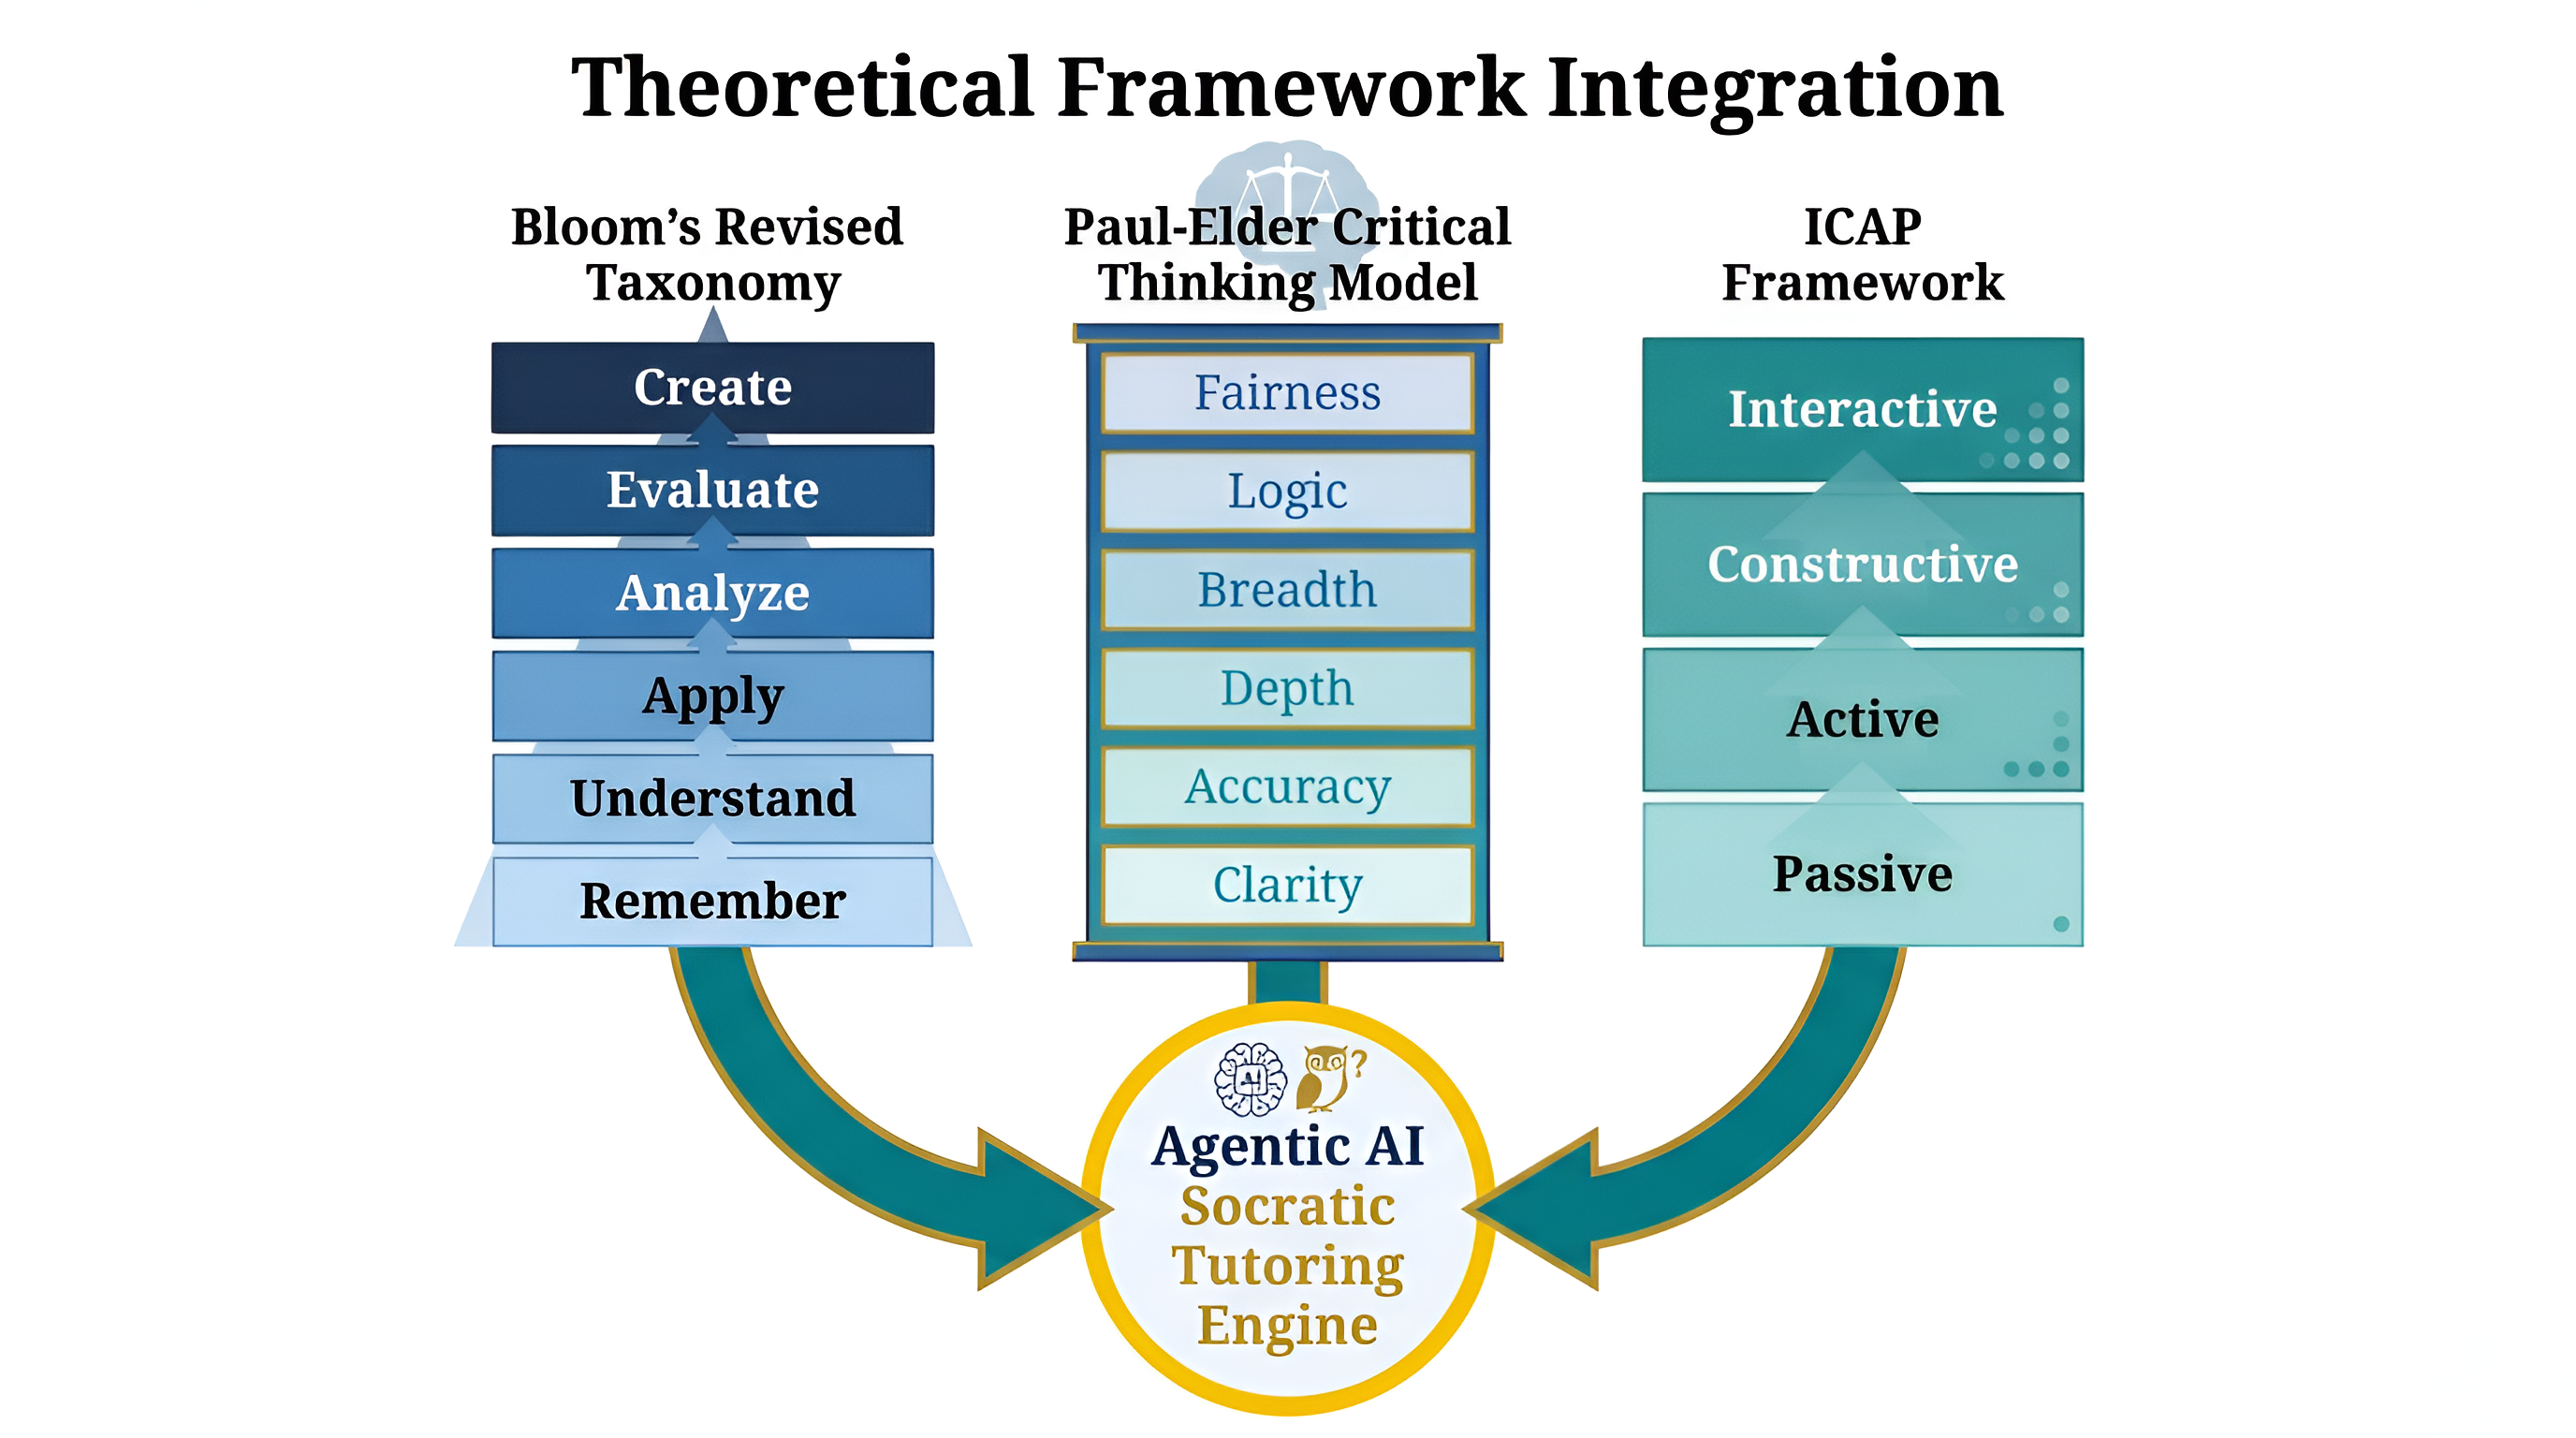
\includegraphics[width=0.88\textwidth]{canvas-image-1-1776007092408.png}
    \caption{ThinkMate theoretical framework linking Bloom's revised taxonomy, the Paul-Elder model, ICAP engagement, and agentic Socratic tutoring.}
\end{figure}

\begin{figure}[H]
    \centering
    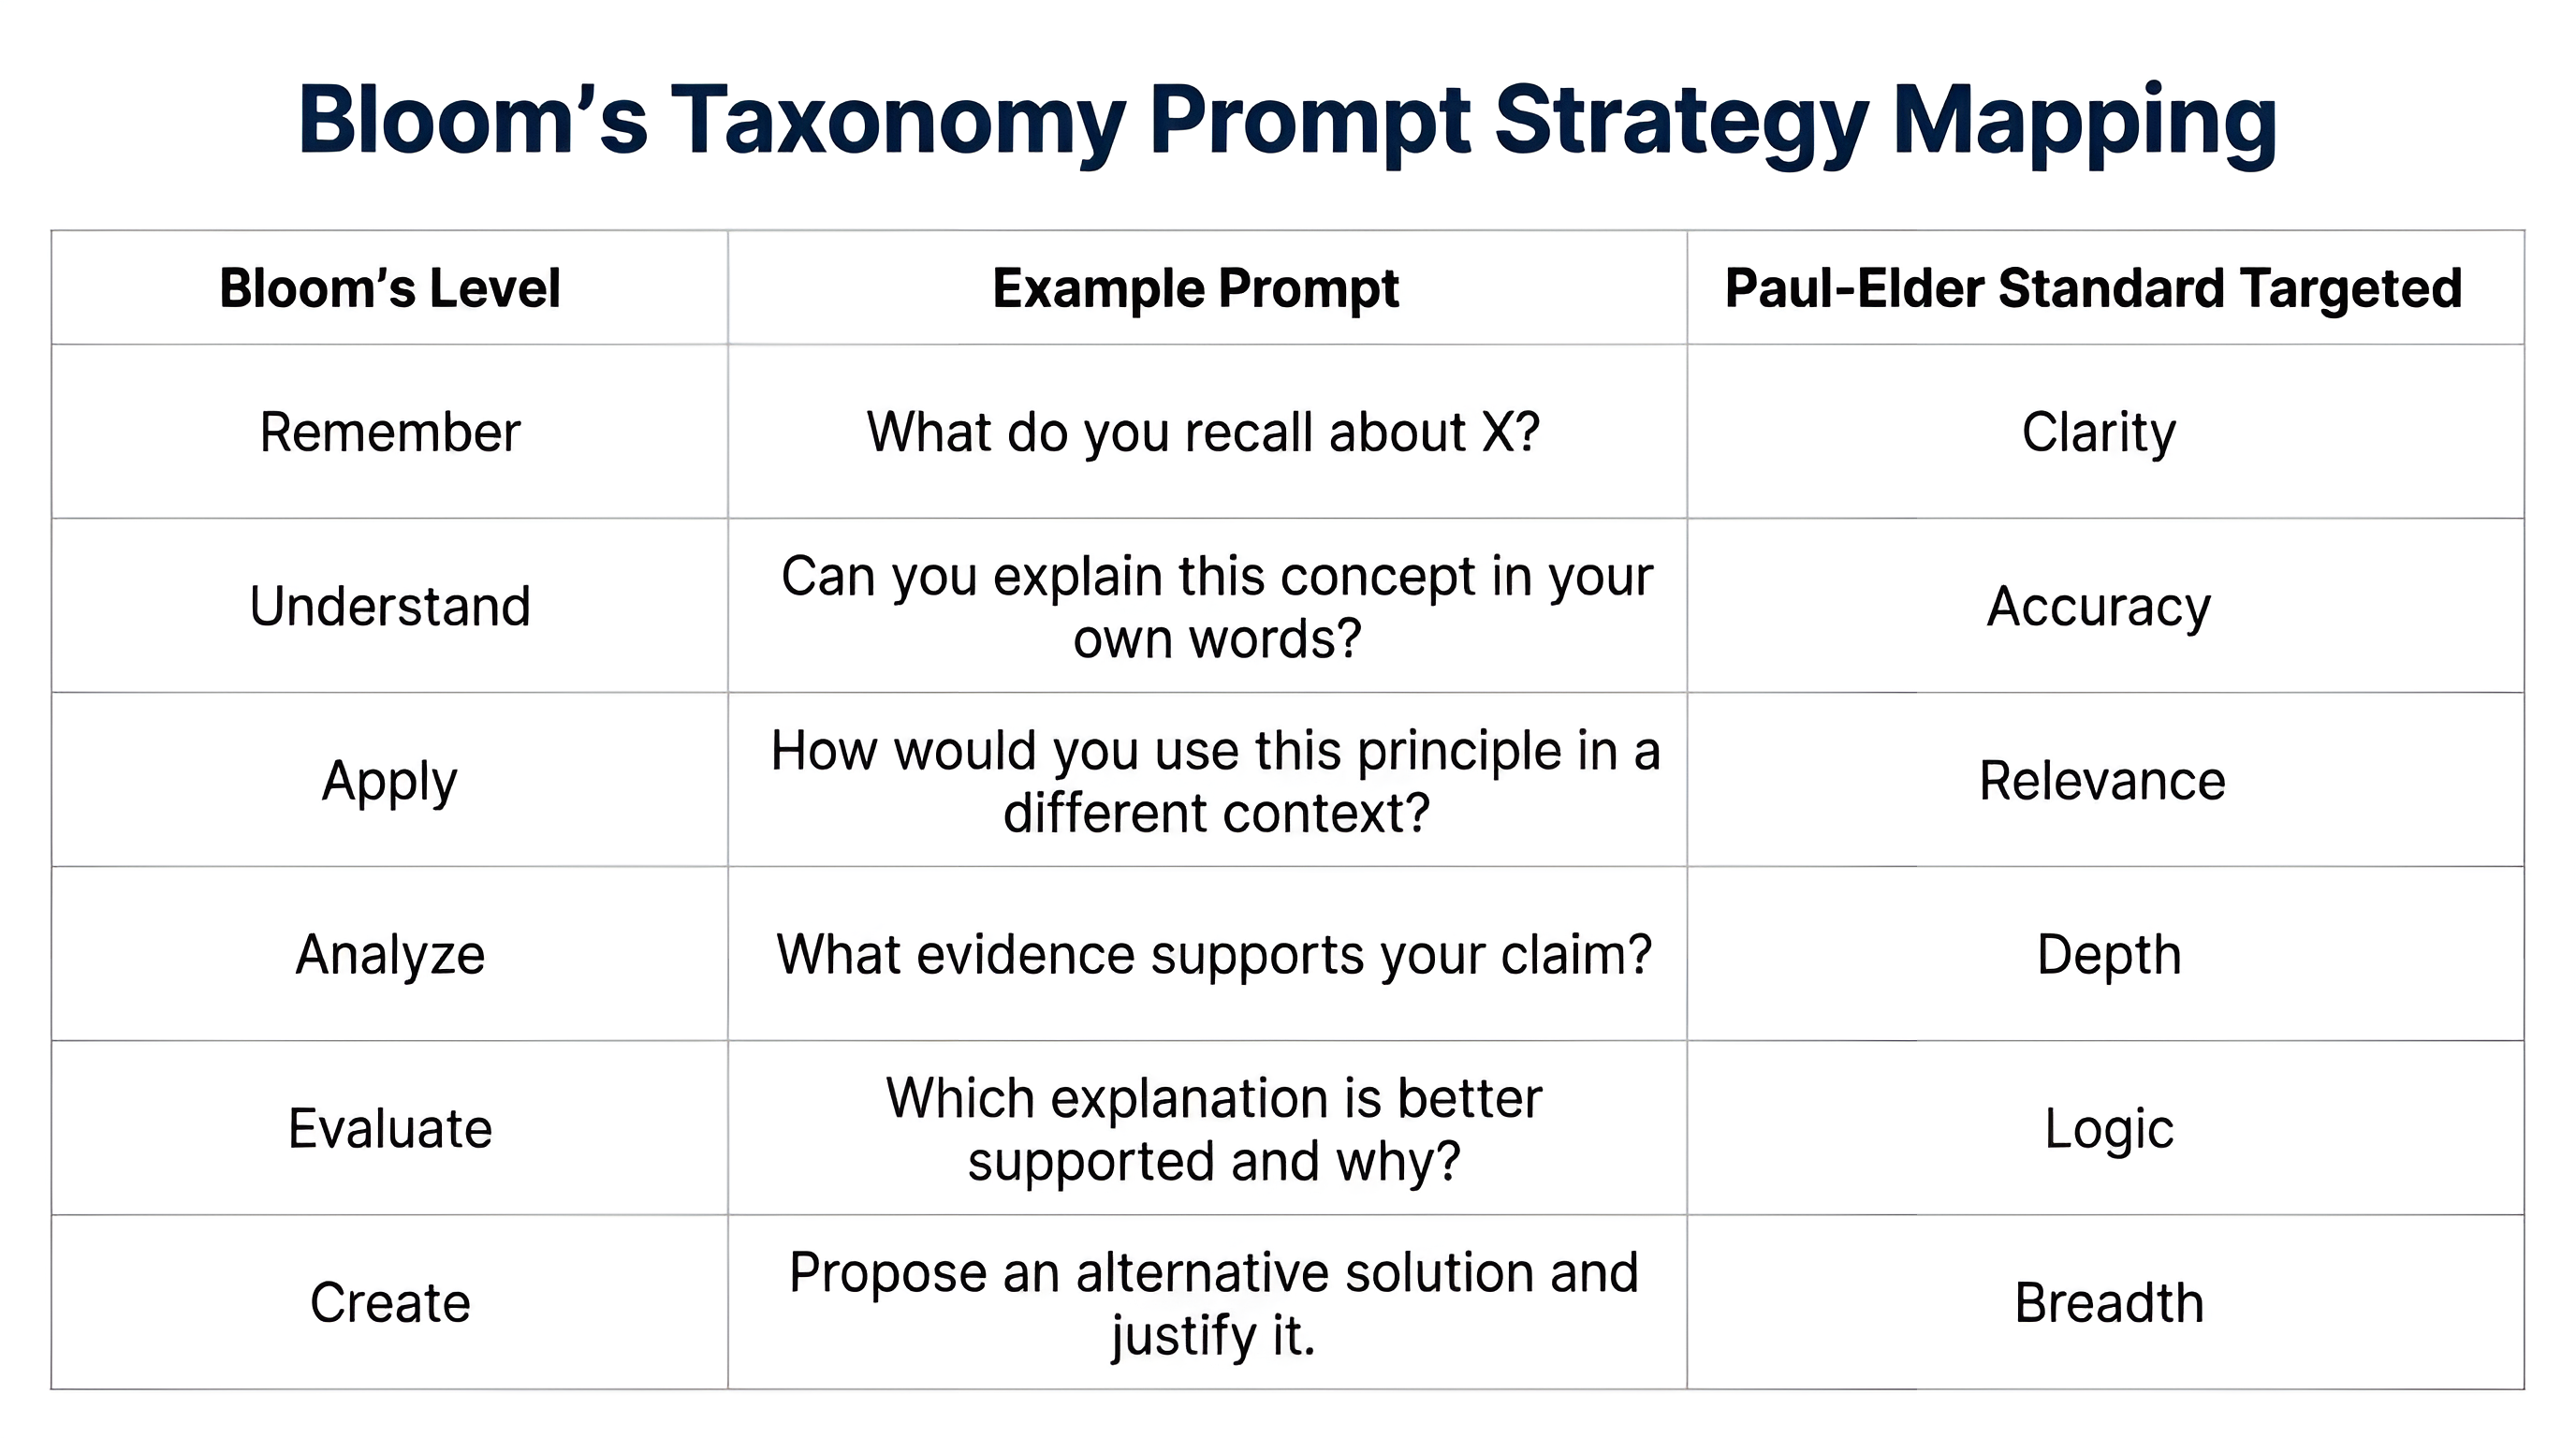
\includegraphics[width=0.88\textwidth]{canvas-image-1-1776007592264.png}
    \caption{Bloom's taxonomy prompt strategy mapping showing the correspondence between cognitive levels, example Socratic prompts, and targeted Paul-Elder intellectual standards.}
\end{figure}

\subsection*{Objectives}
\begin{enumerate}[nosep]
    \item Design and validate a constrained Socratic dialogue architecture that maps Bloom's levels and Paul-Elder standards onto observable tutoring moves for two pilot disciplines.
    \item Build a pilot-ready web platform with two course-specific modules (Engineering and Humanities), prompt controls, instructor dashboards, and dialogue logging.
    \item Evaluate implementation feasibility through recruitment, completion, usability, fidelity, and instructor acceptability metrics in two UAEU pilot courses.
    \item Estimate the effect of ThinkMate on students' course-embedded reasoning quality relative to a matched non-AI guided comparison condition.
    \item Use dialogue logs, fidelity checks, and instructor feedback to generate an evidence-based decision to scale, redesign, or stop.
\end{enumerate}

\subsection*{Research Questions}
\begin{enumerate}[nosep, label={RQ\arabic*.}]
    \item Can ThinkMate be implemented with acceptable feasibility, usability, and instructional fidelity across the two pilot courses?
    \item Do students produce stronger rubric-scored reasoning on matched course tasks when supported by ThinkMate than when using a non-AI guided comparison?
    \item Which usage patterns and fidelity indicators are associated with stronger or weaker reasoning outcomes?
    \item How should positive, null, or mixed findings be interpreted when deciding whether ThinkMate should be scaled, redesigned, or stopped?
\end{enumerate}

\subsection*{Directional Hypothesis}
\textbf{H1.} Relative to the matched non-AI condition, ThinkMate is expected to improve mean blinded rubric-scored reasoning quality on course-embedded tasks, with $d = 0.30$ as the pre-specified minimum practically meaningful effect for informing scale-up decisions.

%% =============================================================================
%%  3. METHODOLOGY
%% =============================================================================
\section{Methodology}

The project employs design-based research (Barab and Squire, 2004) for development with an embedded pilot evaluation randomised within courses. This approach was selected for its capacity for iterative refinement of the platform while still producing a defensible effect estimate within the 8-month grant period.

\subsection*{Phase 1: Co-Design and Protocol Development (May--July 2026)}

The PIs and participating instructors will review course assessments where reasoning quality is an intended outcome and identify two candidate tasks per course that require explanation and judgement rather than factual recall. The primary pilot courses are AERO~590 / MECH~590 (Capstone Engineering Design Project) and PSYC485 (Integrated Capstone). Capstone contexts were selected deliberately: they demand extended justification, synthesis, and reflective decision-making, which align with the reasoning goals of the intervention. The matched tasks within each capstone will be common assessment components that all students complete, such as a design-justification brief in Engineering or a theory-application critique in Psychology, rather than individualized capstone deliverables.

\subsection*{Phase 2: Platform Development (July--September 2026)}

The React front end, FastAPI back end, logging layer, and instructor dashboard will be implemented by the Engineering students. Humanities students will develop discipline-specific prompt libraries, misconception maps, and rubric-linked tutoring moves. Alpha testing will be conducted internally; beta testing will include red-team prompts designed to detect answer leakage or weak pedagogical moves before the pilot goes live.

\subsubsection*{Constrained Move-Selector Architecture}

The core pedagogical component is a rule-based move selector that operates independently of the language-generation layer. The selector maintains a finite action space of six moves: \textit{clarification request}, \textit{evidence probe}, \textit{assumption probe}, \textit{counterview challenge}, \textit{synthesis prompt}, and \textit{reflection cue}. On each turn, the system first classifies the student's prior response using an LLM-based classifier along two dimensions: (a)~the Bloom's cognitive level exhibited (with emphasis on the boundary between understanding and analysing) and (b)~detected weakness in Paul-Elder standards (e.g., low specificity signals a clarity gap; unsupported claims signal a depth gap). The classifier output is mapped through a decision matrix to select the next pedagogical move. Only after the move is selected does the system invoke the LLM to generate the natural-language realisation of that move, using a constrained prompt template that specifies the move type, the targeted standard, and explicit instructions to withhold direct answers. A separate safeguard pass audits the generated response for answer leakage or premature closure before delivery.

\subsubsection*{ICAP Engagement Classification}

The learner-state layer classifies each student turn using keyword density, response length, and an LLM-based semantic check. Short acknowledgements and single-sentence restatements are classified as passive; self-generated explanations with new reasoning are classified as constructive; and responses that substantively revise a prior position after a challenge prompt are classified as interactive. Classification accuracy will be validated against human-coded samples during alpha testing, with a target agreement of at least 80\% before the pilot proceeds. These ICAP-level signals are logged per turn and analysed as candidate mechanisms behind positive or null results.

\subsubsection*{Content Accuracy Safeguards}

Beyond answer-leakage detection, the system mitigates LLM hallucination risk through retrieval-augmented generation (RAG) grounded in instructor-vetted course materials stored in the vector database. Socratic questions are generated from verified disciplinary content rather than unconstrained LLM knowledge. During beta testing, a sample of generated questions will be reviewed by both PIs for factual accuracy, and any systematic error patterns will be corrected in prompt templates before the pilot launches.

\subsection*{Phase 3: Pilot Evaluation Design}

The pilot evaluation uses two matched reasoning tasks per course and a counterbalanced crossover design. Students are randomized to sequence A or B. In Task~1, sequence A uses ThinkMate while sequence B completes a non-AI guided activity; in Task~2, conditions are switched. The non-AI comparison condition was deliberately designed to be strong: a structured guided worksheet which mirrors the reasoning sequence of the AI condition (initial claim, evidence, assumption check, counterargument, revision, reflection) is delivered through the LMS in same activity window. Facilitators provide only procedural clarification, not individualized Socratic probing.

The target sample is approximately 80 students across two courses (acceptable range: 60--100). The minimum effect of interest, $d = 0.30$, was selected on the basis that effects below this threshold would not justify the operational cost of institutional scale-up and is consistent with the lower bound of effects reported in structured AI-tutoring interventions (Kestin et al., 2025). Assuming $\alpha = 0.05$ (two-tailed), a within-subject correlation of $r = 0.50$, and two measurement occasions per student in the crossover design, a paired-samples comparison yields approximately 80\% power to detect $d = 0.30$. The assumed correlation of $r = 0.50$ reflects the expectation that reasoning quality on two tasks within the same capstone course and semester will be moderately stable within individuals; if the true correlation is lower ($r = 0.30$), power at $n = 80$ would decrease to approximately 65\%, reinforcing the framing of this project as a pilot estimation study rather than a definitive efficacy trial. The acceptable range of 60--100 students corresponds to power of approximately 60\%--88\% across plausible correlation values.

The primary outcome is reasoning quality on authentic course artifacts scored by two raters blinded to condition, student identity, and sequence using an analytic rubric derived from Paul-Elder standards. Inter-rater reliability will be assessed using intraclass correlation coefficients (ICC, two-way random, absolute agreement); a minimum ICC of 0.70 is required before scoring proceeds, and if the threshold is not met after calibration a third rater will adjudicate discrepant scores. Secondary outcomes include consent rate, completion rate, dialogue depth, safeguard fidelity, System Usability Scale (SUS; Brooke, 1996) scores, and instructor acceptability. The analysis plan, including primary model specification and decision thresholds, will be pre-registered on OSF before the pilot launches. The primary analysis uses a linear mixed-effects model with student as a random effect and condition, task, course, and sequence as fixed effects. Secondary outcomes are treated as exploratory and will not be adjusted for multiplicity. Effect sizes and 95\% confidence intervals are emphasized alongside $p$-values. Qualitative data from post-pilot interviews and focus groups will be analysed using reflexive thematic analysis (Braun and Clarke, 2006) to identify patterns in student experience and instructor perceptions.

Bias control is built into the protocol. Time-on-task is logged in both conditions to separate engagement duration from pedagogical effect. The crossover structure probes novelty effects: if gains attenuate on the second task, an AI excitement artefact is implicated. Conversely, if students who receive ThinkMate first show improved performance on the second non-AI task, a carryover learning effect may be present; the linear mixed model includes a sequence-by-condition interaction term to detect and quantify such asymmetric transfer. Self-selection is addressed by randomizing within intact courses. The project does not assume positive results; null or mixed outcomes will be interpreted through the lens of prompt design, task alignment, and usage patterns as cautioned by Bastani et al.\ (2024) and Thoeni and Fryer (2025).

Feasibility is protected by a minimal viable staffing model. If positions are filled late, the pilot proceeds with one Engineering developer, one Humanities content lead, and one graduate RA under direct faculty supervision. English is the pilot language; Arabic support is a planned post-pilot extension. If the MVP is not functional by August 20, the pilot will proceed with a reduced feature set limited to one dialogue pathway per course and a text-only interface, deferring the instructor dashboard to post-pilot. Students will receive a written information sheet explaining the study purpose, describing AI interaction logging, and confirming that participation does not affect course grades. Consent will be obtained electronically before the first session; students who decline or withdraw receive the structured guided worksheet condition for both tasks, ensuring no disadvantage. All study data will be stored on UAEU-hosted secure servers; dialogue logs and survey responses will be pseudonymised at collection and retained for five years following the project's conclusion in accordance with UAEU research data management policy and the UAE Federal Decree-Law No.\ 45/2021 on the Protection of Personal Data.

\subsection*{Risk and Mitigation Overview}

\begin{tabularx}{\textwidth}{|L{4.5cm}|X|}
\hline
\rowcolor{lightGray}
\textbf{Risk} & \textbf{Mitigation} \\ \hline
LLM API costs exceed budget & Set usage caps, monitor tokens weekly, and retain an open-source fallback option for selected functions. \\ \hline
Tutor gives direct answers or weak guidance & Red-team prompts before launch, sample dialogue audits during the pilot, and fallback template prompts if safeguard fidelity drops. \\ \hline
Low student recruitment for the pilot & Recruit through multiple eligible sections and widen participation if one section under-enrols. \\ \hline
Ethics approval is delayed & Submit in Week 1 after informal consultation with UAEU Research Ethics Committee. If approval is not received by September 15, pilot deployment will be delayed by two weeks with milestones shifted accordingly within the grant period. \\ \hline
Technical issues appear during the pilot & Keep a buffer between beta testing and launch and provide direct technical support during pilot weeks. \\ \hline
Student team attrition & Cross-train students, document workflows clearly, and store work in shared repositories. \\ \hline
LLM generates factually inaccurate Socratic questions & Ground generation in RAG over vetted course materials; PI review of sampled questions during beta testing; fallback to curated template prompts for high-risk topics. \\ \hline
LLM provider changes API terms or pricing mid-project & Budget includes token-cap monitoring; architecture allows substitution of an open-source model (e.g., Llama) for non-latency-sensitive functions. \\ \hline
Pilot course is not offered or under-enrols in Fall 2026 & Confirm course scheduling with department chairs by M1; identify one backup section per college that could serve as an alternative pilot site. \\ \hline
\end{tabularx}

\begin{figure}[H]
    \centering
    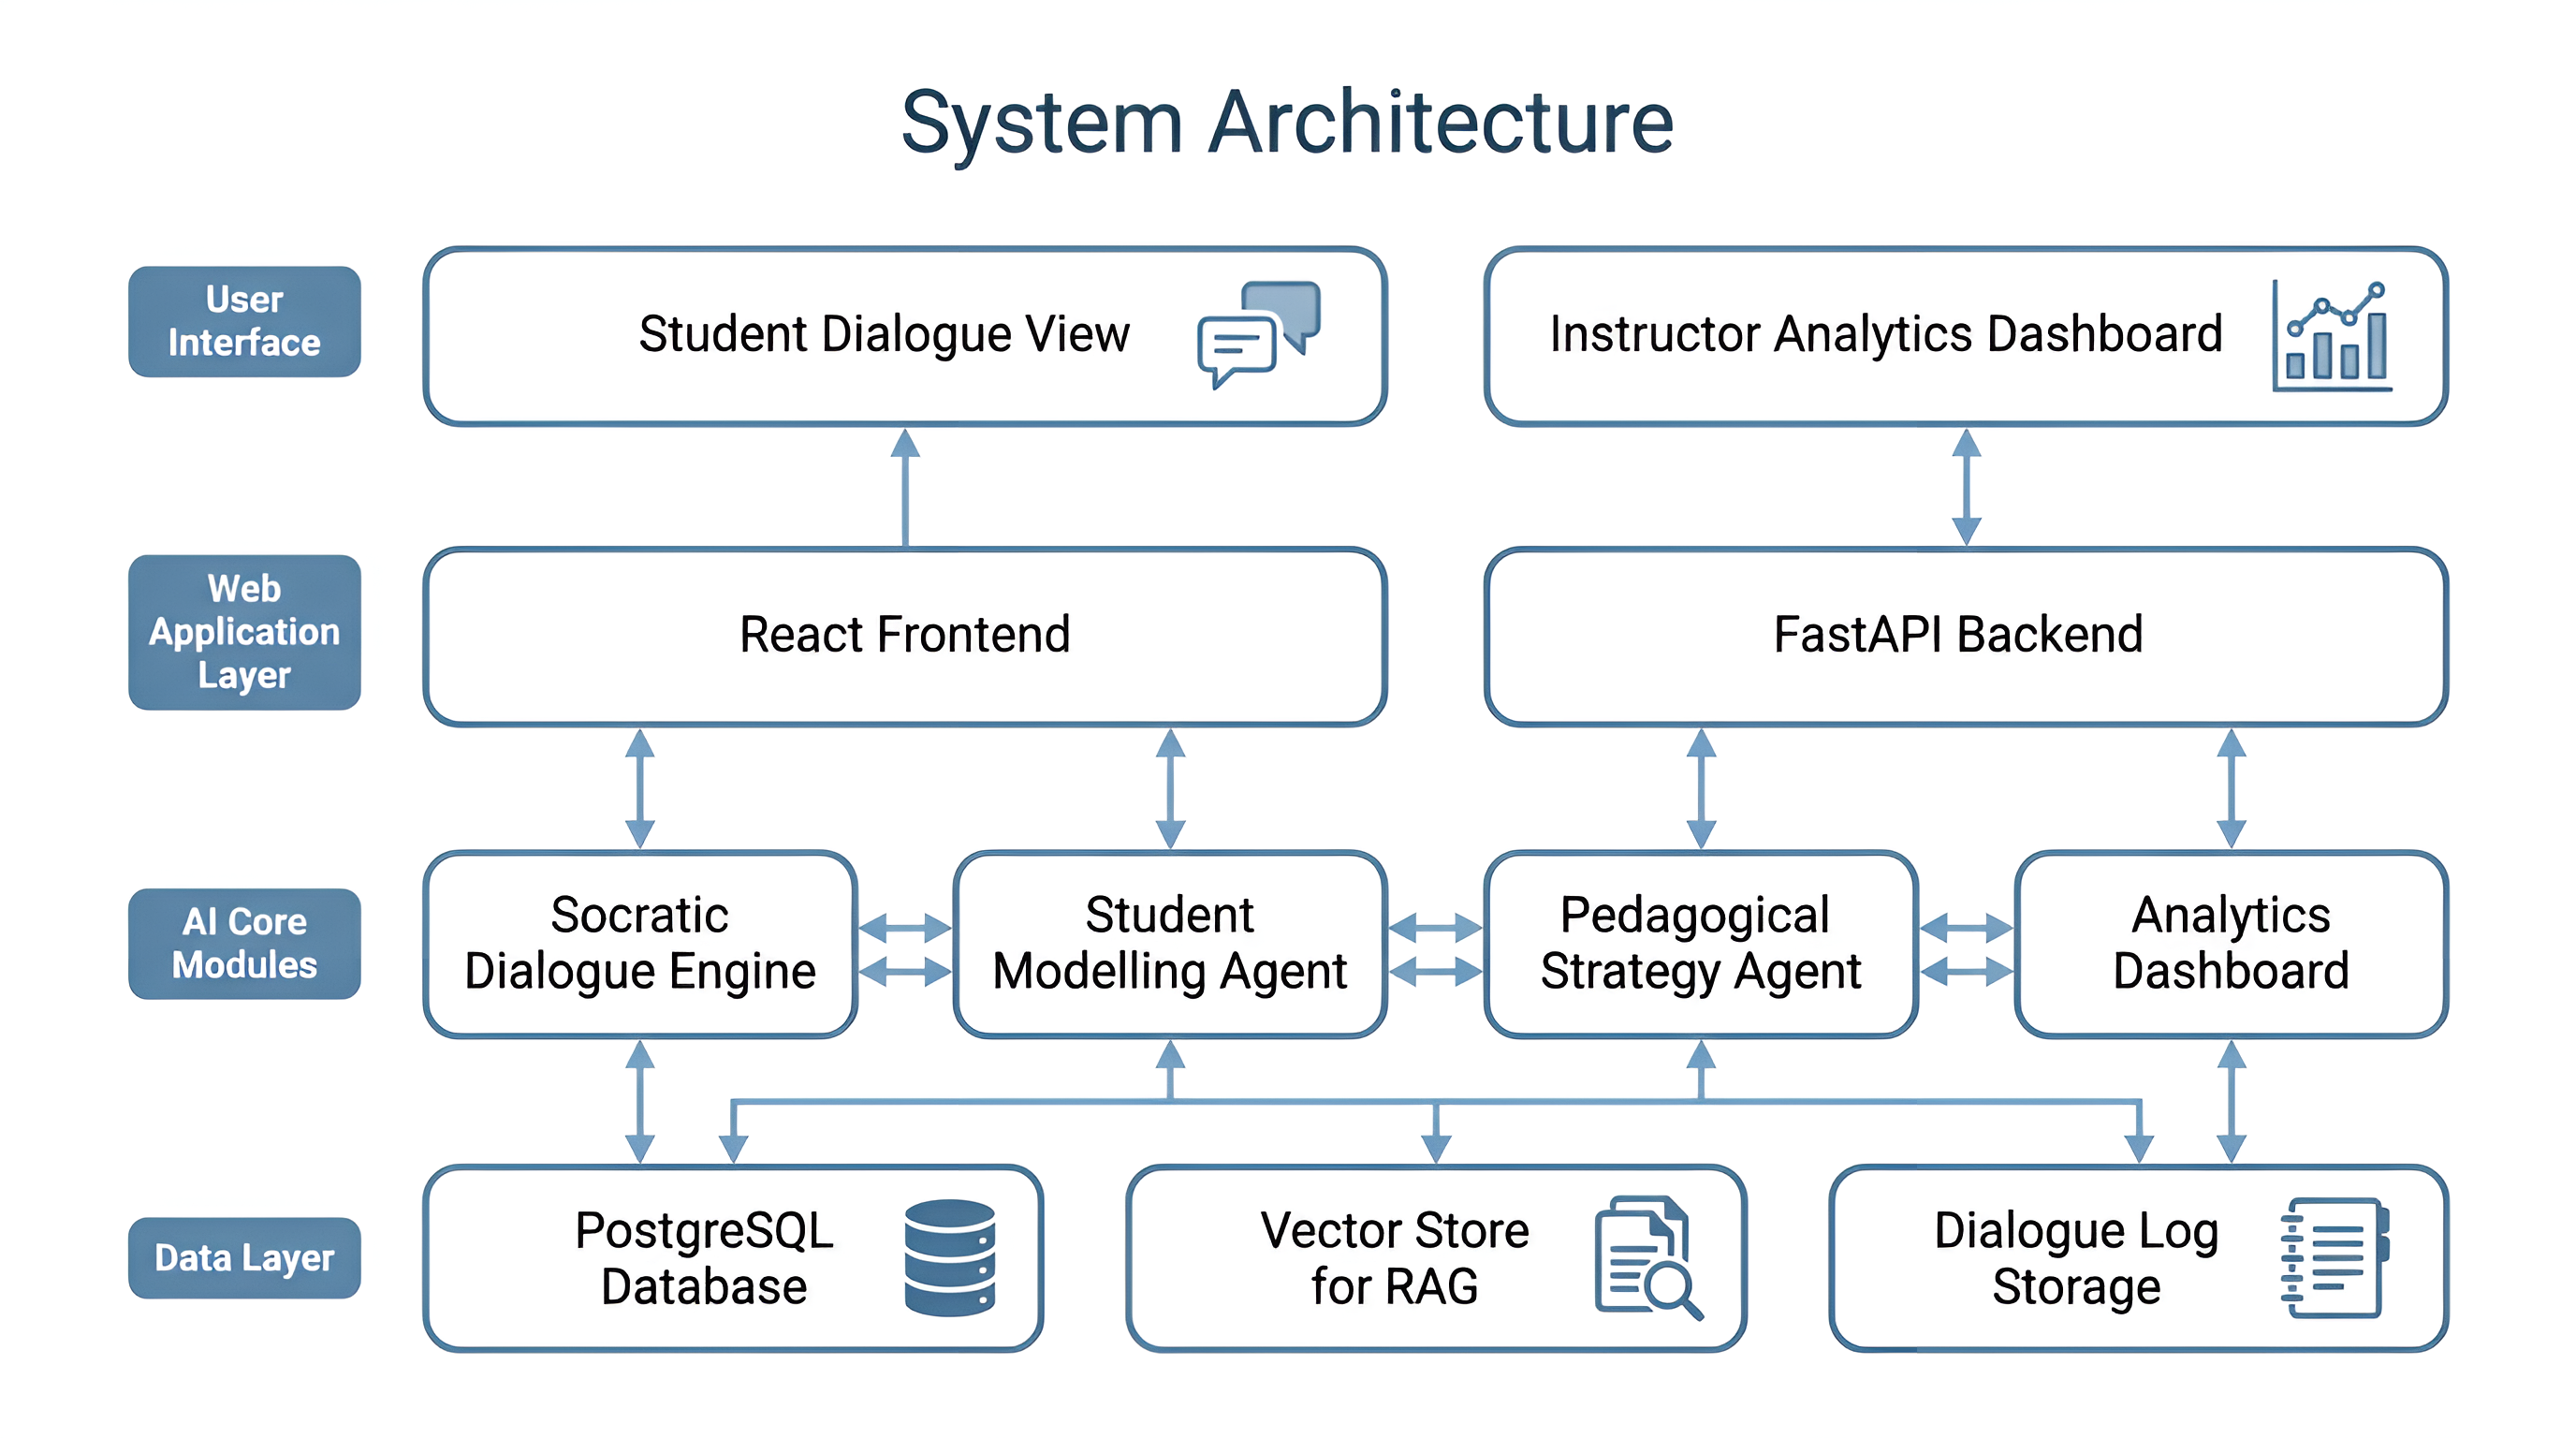
\includegraphics[width=0.88\textwidth]{canvas-image-1-1776007169497.png}
    \caption{System architecture showing the four-layer platform design with user interface, web application, AI core modules, and data storage layers.}
\end{figure}

\begin{figure}[H]
    \centering
    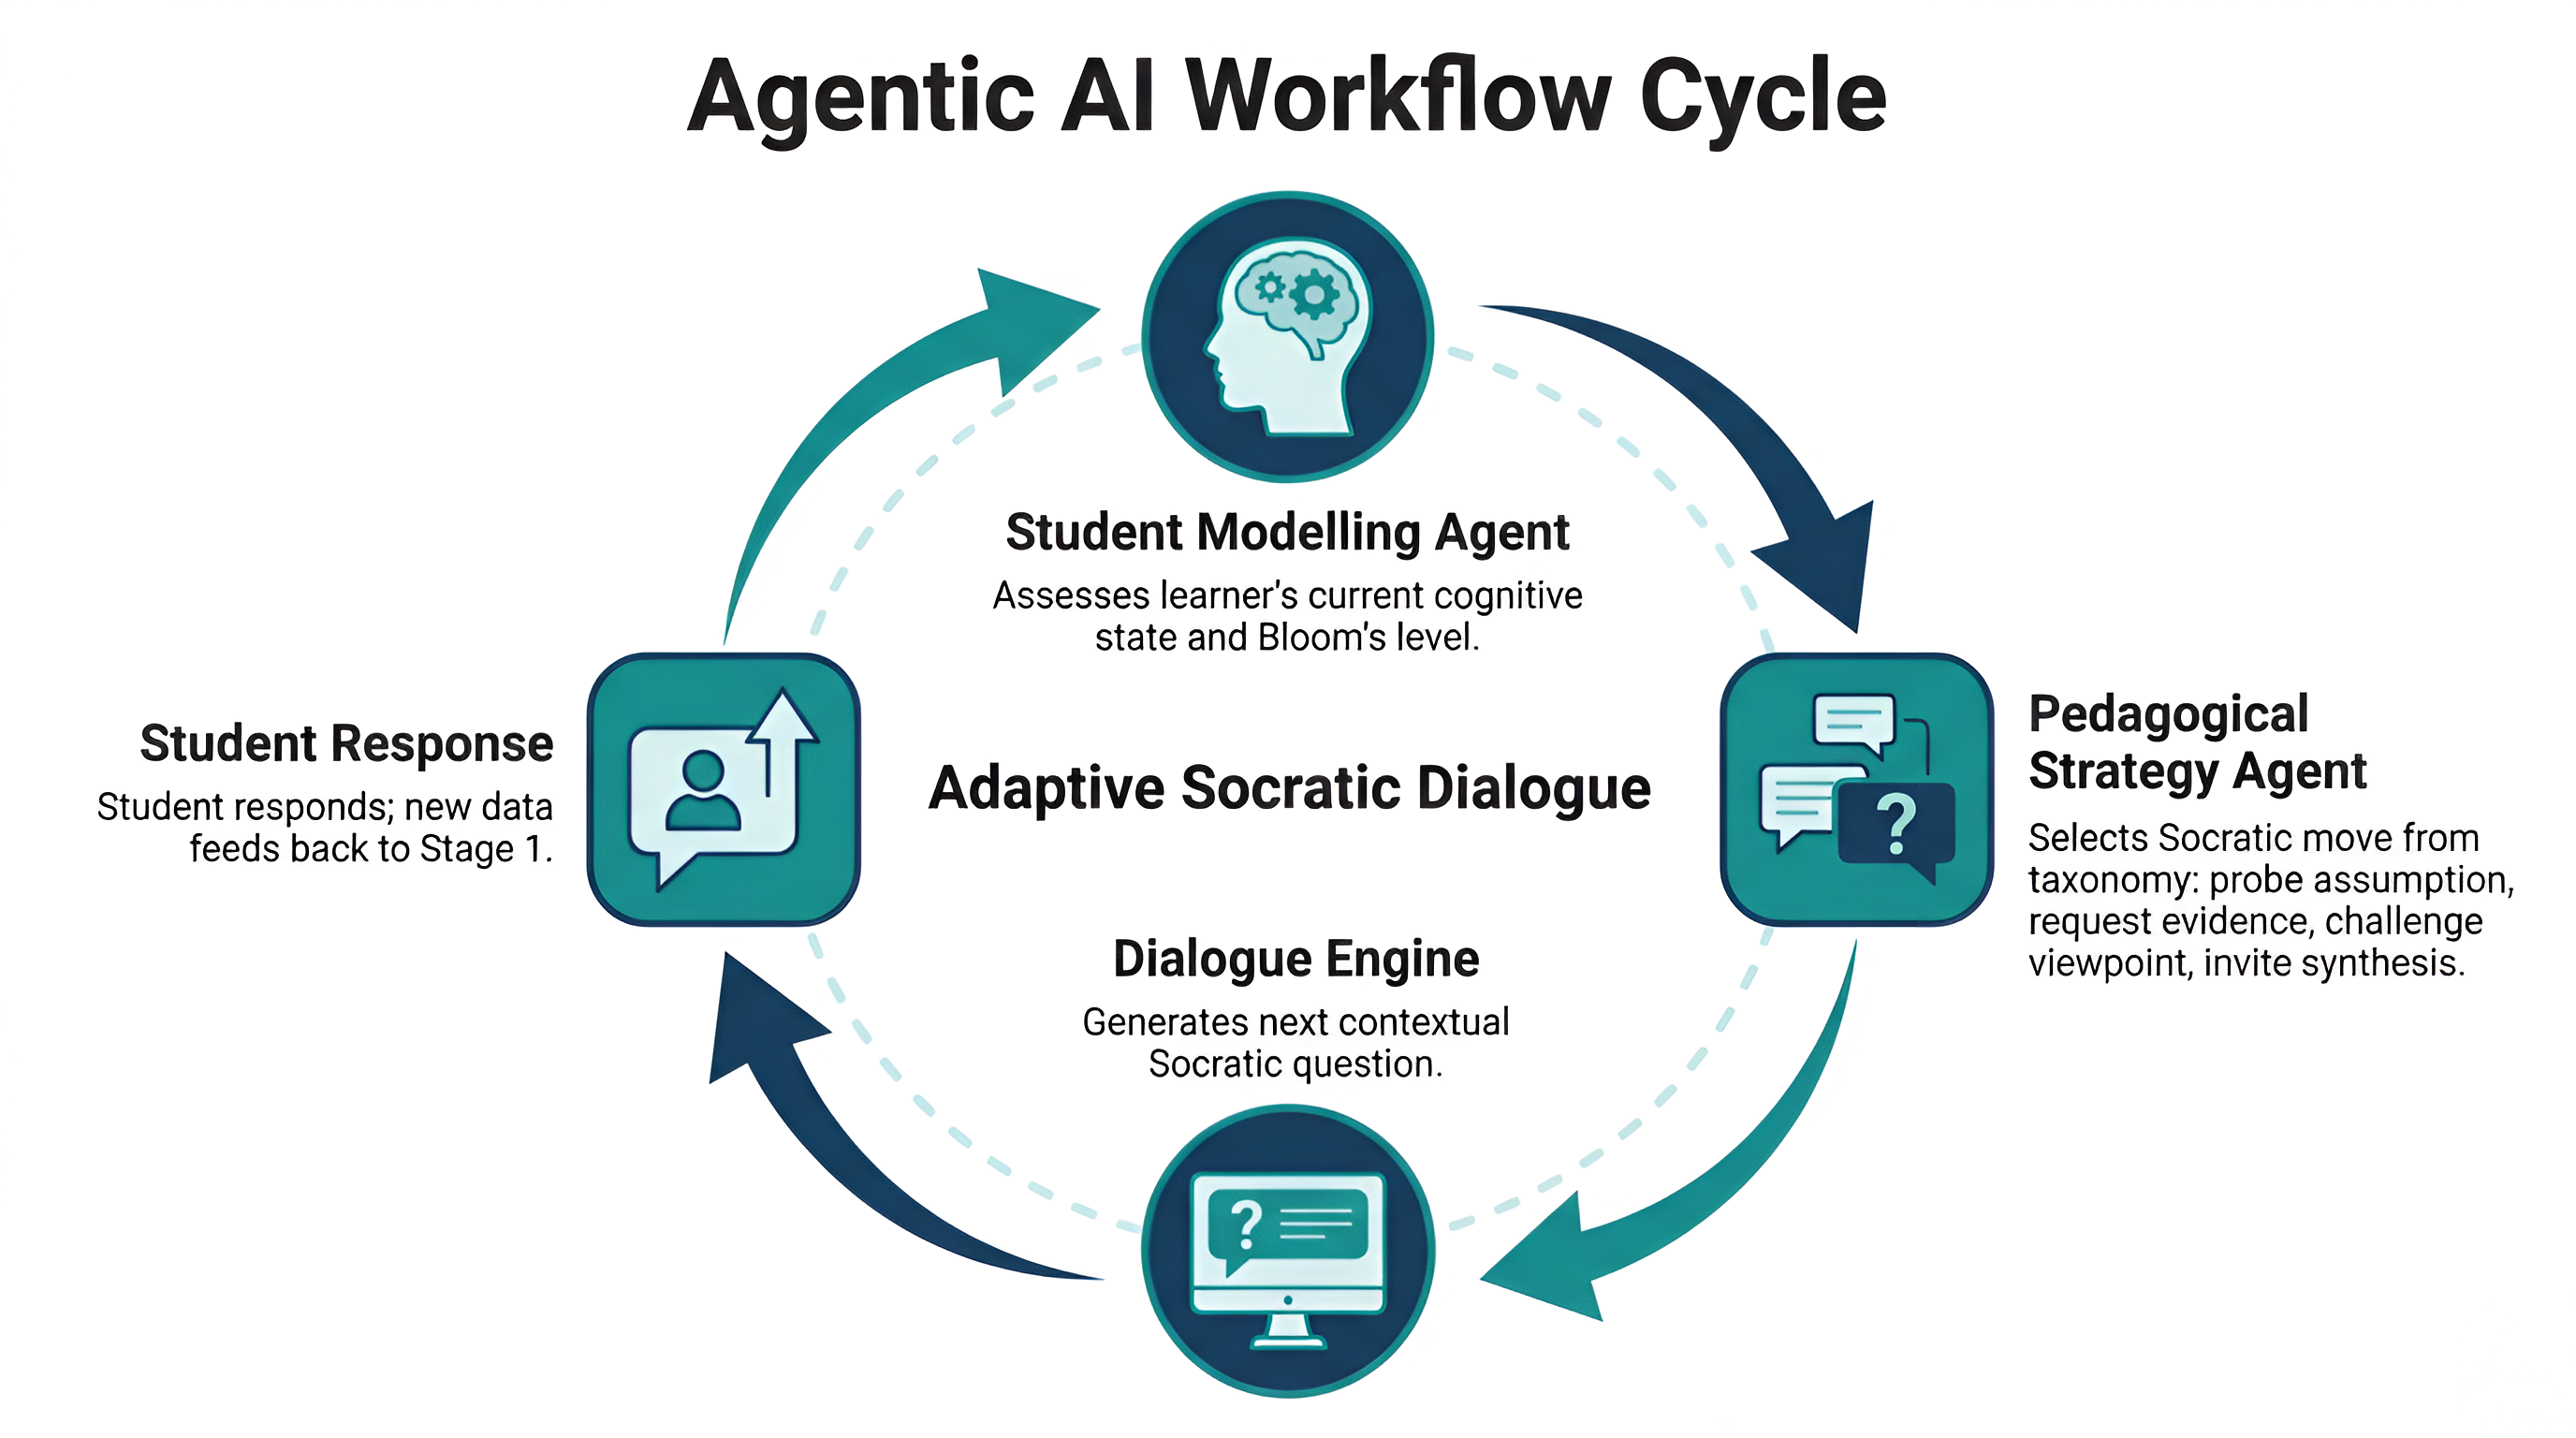
\includegraphics[width=0.85\textwidth]{canvas-image-1-1776007245564.png}
    \caption{Agentic AI workflow cycle showing the adaptive Socratic dialogue loop between student modelling, strategy selection, dialogue generation, and student response.}
\end{figure}

\begin{figure}[H]
    \centering
    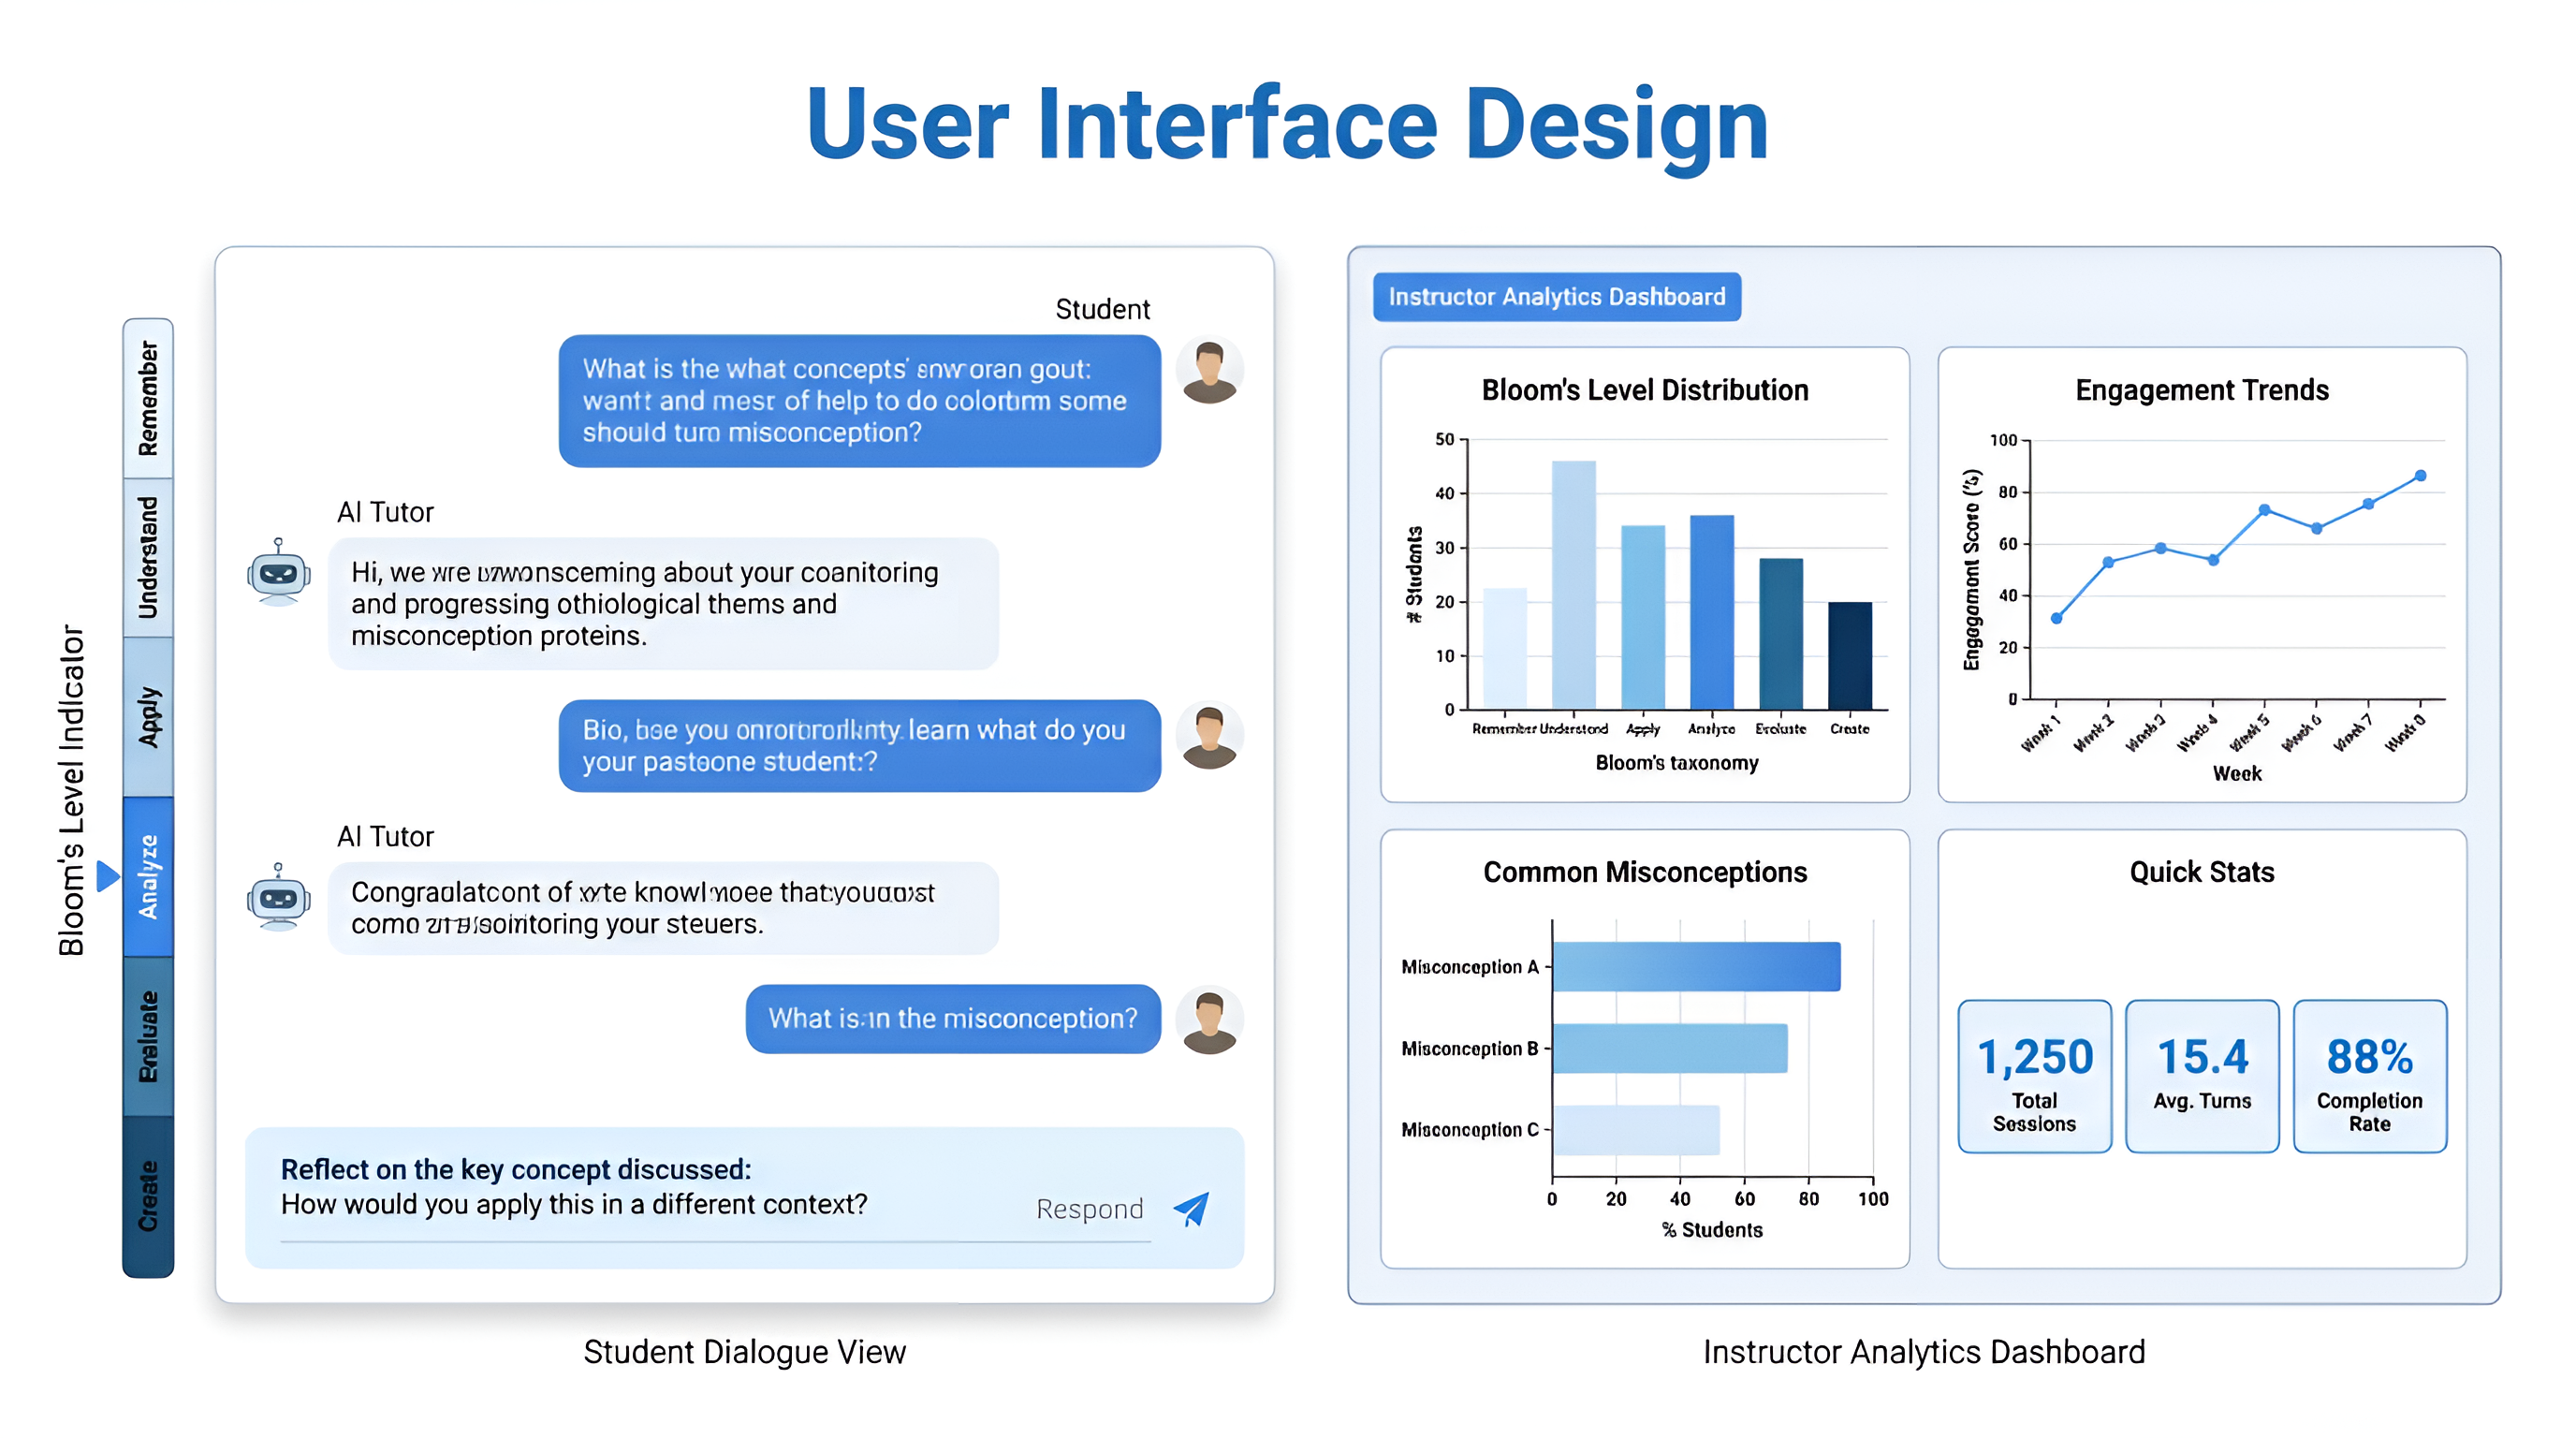
\includegraphics[width=0.88\textwidth]{canvas-image-1-1776007328620.png}
    \caption{User interface wireframe mockup showing the student dialogue view with Bloom's level indicator (left) and the instructor analytics dashboard (right). Final interface text will reflect actual Socratic dialogue content.}
\end{figure}

\begin{figure}[H]
    \centering
    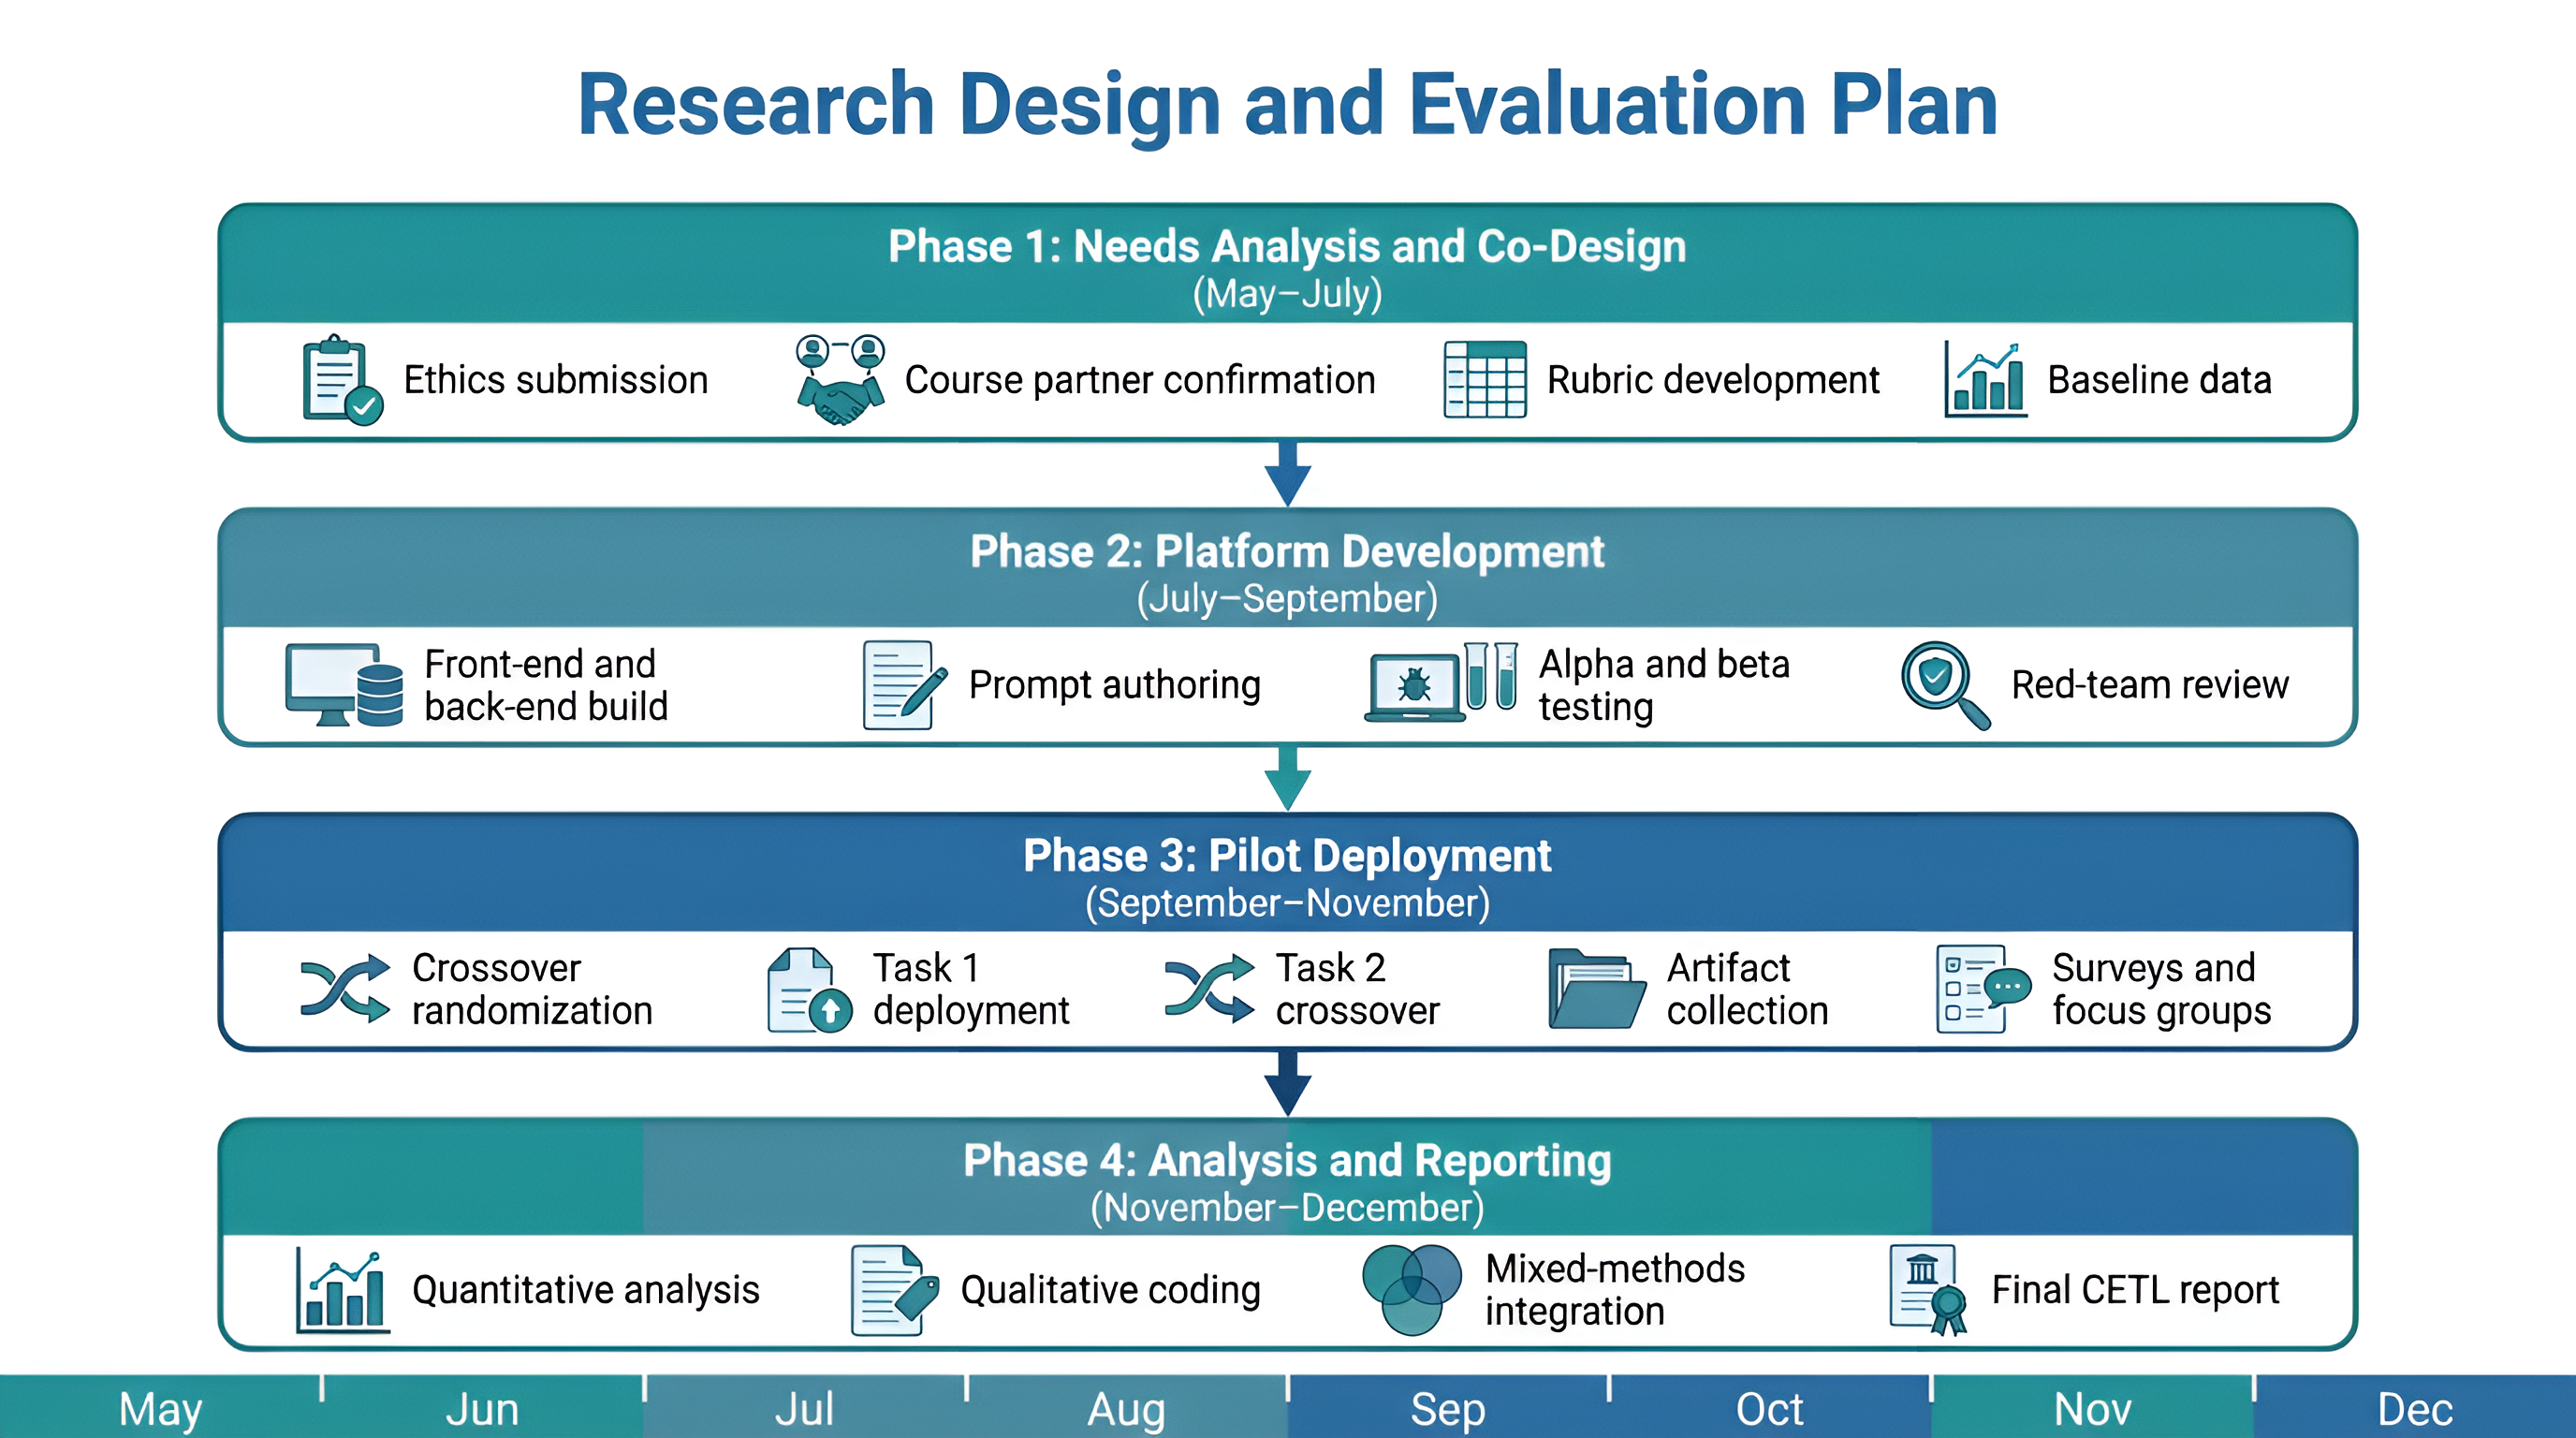
\includegraphics[width=0.88\textwidth]{canvas-image-1-1776007477227.png}
    \caption{Research design and evaluation plan showing the four-phase methodology from needs analysis through final reporting.}
\end{figure}

%% =============================================================================
%%  4. TIME SCHEDULE
%% =============================================================================
\section{Time Schedule for the Project Tasks}

\begin{tabularx}{\textwidth}{|X|C{1.2cm}|C{1.2cm}|C{1.2cm}|C{1.2cm}|}
\hline
\rowcolor{lightGray}
\textbf{Tasks} & \textbf{Q1} & \textbf{Q2} & \textbf{Q3} & \textbf{Q4} \\ \hline
1- Team onboarding, literature update, and course partner confirmation & X & & & \\ \hline
2- Ethics application and protocol finalisation & X & & & \\ \hline
3- Co-design of pilot tasks and scoring rubrics & X & X & & \\ \hline
4- System architecture, UI/UX, and logging design & X & X & & \\ \hline
5- Platform back-end and safeguard implementation & & X & & \\ \hline
6- Platform front-end and dashboard development & & X & & \\ \hline
7- Discipline-specific prompt and content authoring & & X & & \\ \hline
8- Alpha testing, beta testing, and red-team review & & X & & \\ \hline
9- Pilot Task 1 deployment in both courses & & & X & \\ \hline
10- Pilot Task 2 crossover deployment & & & X & \\ \hline
11- Artifact scoring, surveys, logs, and focus groups & & & X & \\ \hline
12- Quantitative and qualitative analysis & & & & X \\ \hline
13- Scale-up decision memo and CETL final report & & & & X \\ \hline
14- Poster design and dissemination preparation & & & & X \\ \hline
15- Journal or conference manuscript preparation & & & X & X \\ \hline
\end{tabularx}

\begin{figure}[H]
    \centering
    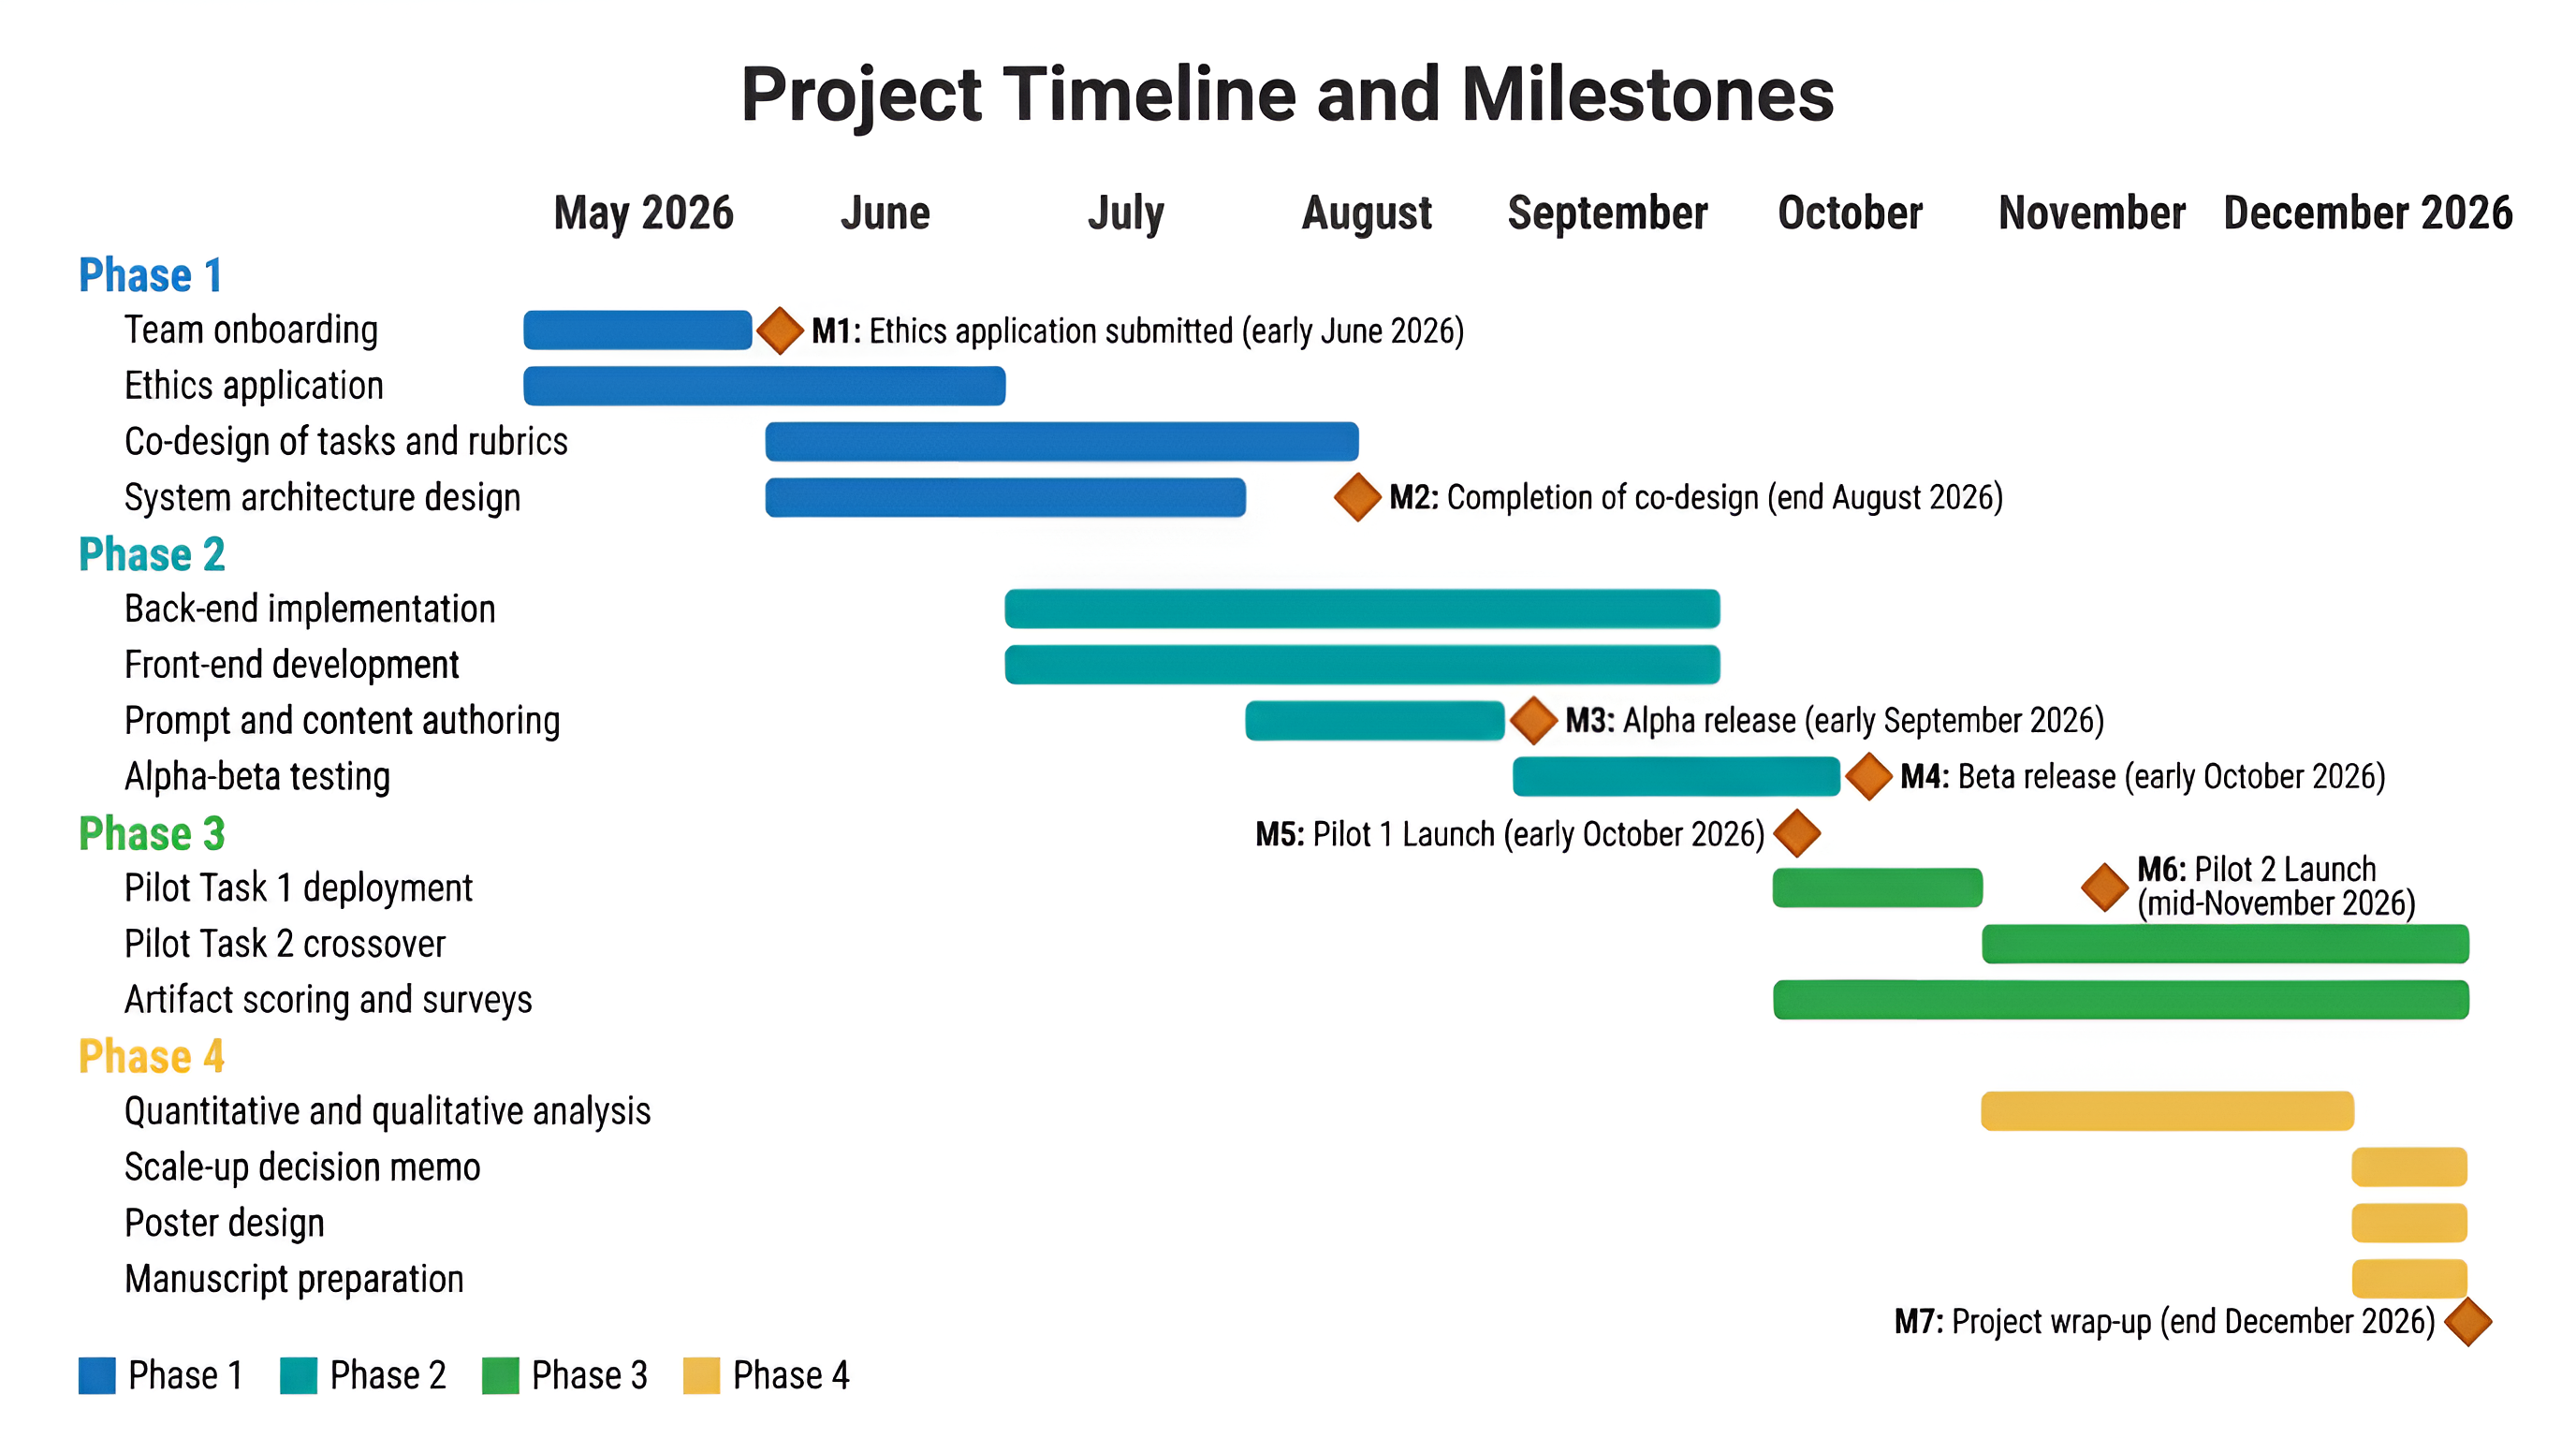
\includegraphics[width=0.88\textwidth]{canvas-image-1-1776007820922.png}
    \caption{Project timeline and milestones for the period from May 2026 to December 2026.}
\end{figure}

\subsection*{Milestone Checkpoints}

\begin{tabularx}{\textwidth}{|L{4.2cm}|L{2.2cm}|X|}
\hline
\rowcolor{lightGray}
\textbf{Milestone} & \textbf{Target Date} & \textbf{Success Criterion} \\ \hline
M1: Ethics submitted and course partners confirmed & Early June 2026 & Pilot courses selected, tasks identified, and ethics package submitted. \\ \hline
M2: Co-design of tasks and rubrics complete & Late August 2026 & Prompt safeguards, scoring rubrics, and evaluation plan reviewed by both PIs. \\ \hline
M3: Alpha release of prototype & Early September 2026 & Core dialogue, logging, and dashboard components working in test mode. \\ \hline
M4: Beta release and red-team testing complete & Early October 2026 & Answer-leakage and usability issues addressed before pilot launch. \\ \hline
M5: Pilot Task~1 launched & Early October 2026 & Students complete the first crossover task in both courses. \\ \hline
M6: Pilot Task~2 and scoring complete & Mid-November 2026 & Artefacts, interviews, focus groups, and scoring dataset completed. \\ \hline
M7: Final report and project wrap-up & End of December 2026 & Final CETL report and evidence-based next-step recommendation submitted. \\ \hline
\end{tabularx}

%% =============================================================================
%%  5. OUTCOMES AND NOVELTY STATEMENT
%% =============================================================================
\section{Outcomes and Novelty Statement}

The project is expected to produce five direct outputs: a functional ThinkMate prototype, two discipline-specific pilot modules, a pilot evaluation report, a final CETL report, and at least one scholarly dissemination output. The project treats product delivery and educational evidence as equally necessary outcomes because a prototype without credible evaluation would not justify broader institutional adoption. The primary educational benchmark is $d = 0.30$ on blinded rubric-scored reasoning quality, as defined in H1.

\subsection*{Success Targets}

Feasibility targets are at least 60 consenting students, at least 80\% completion, a mean SUS score of 68 or above, and at least 85\% fidelity on sampled dialogues for the no-direct-answer safeguard. The main educational signal is a positive effect of $d \geq 0.30$ on blinded rubric-scored reasoning quality. Effect sizes and confidence intervals are prioritized over significance alone.

\subsection*{Novelty Statement}

ThinkMate separates a constrained pedagogical-move selector from the LLM generation layer, enforces turn-level answer-leakage audits, and logs Paul-Elder-aligned move tags and ICAP engagement states in a live higher-education pilot. It is the first system at UAEU to embed these safeguards into Socratic dialogue and evaluate them against a matched non-AI comparison through blinded scoring of authentic course reasoning tasks.

Null or mixed outcomes will still be scientifically useful. The project will identify whether bottlenecks lie in prompt design, task alignment, student use patterns, or discipline-specific fit. If the pilot meets its thresholds, the final report includes a maintenance plan and phased scale-up proposal. If thresholds are not met, the report provides a structured stop or redesign recommendation.

\subsection*{Outcome Interpretation Matrix}

\begin{tabularx}{\textwidth}{|L{3.5cm}|X|L{3.8cm}|}
\hline
\rowcolor{lightGray}
\textbf{Observed Pattern} & \textbf{Interpretation} & \textbf{Decision} \\ \hline
Feasible and positive effect $\geq d = 0.30$ & The system appears ready for a larger confirmatory study or a limited scale-up in closely matched courses. & Scale cautiously and preserve the same safeguard and scoring logic. \\ \hline
Feasible but effect near zero & The platform is usable, but the current design is not yet producing enough educational value to justify expansion. & Redesign prompts, task alignment, or comparison structure before any further roll-out. \\ \hline
Mixed effects across courses or only under high-fidelity use & The intervention likely has boundary conditions rather than a general effect. & Narrow the scope to the course types or usage profiles where the mechanism appears credible. \\ \hline
Low feasibility regardless of effect direction & Operational weakness, not pedagogy alone, is the main blocker. & Stop scale-up and fix implementation before any further efficacy claims. \\ \hline
\end{tabularx}

% Figure removed: expected-outcome bar charts were replaced by the Outcome
% Interpretation Matrix above, which communicates decision logic without
% presenting speculative data points.

%% =============================================================================
%%  6. RELEVANCE TO TEACHING AND LEARNING
%% =============================================================================
\section{Relevance to Teaching and Learning}

This project addresses a clear teaching and learning need at UAEU: students have limited access to sustained, individualised questioning which helps them explain assumptions, test evidence, and revise incomplete reasoning. In classes of 40--80 students, such support is difficult to provide through instructor time alone. As the literature review demonstrates, the gap between content knowledge and applied reasoning persists across both STEM and humanities disciplines.

ThinkMate responds to that constraint in a student-centred manner. Each learner receives a different sequence of prompts based on response quality, Bloom's level, and detected misconceptions. Hence, AI is used here as a structured pedagogical support system rather than a shortcut for content generation. The adaptive dialogue is designed to push students toward constructive and interactive engagement rather than passive reception.

The interdisciplinary value is central rather than decorative. An Engineering-only team could build the technical stack but would not ensure educationally valid Socratic questioning or defensible CT assessment. A Humanities-only team could design the pedagogical logic but would not deliver the agentic architecture and deployment environment respectively. ThinkMate depends on both colleges because platform logic and educational logic must be designed together. The project is aligned with the UAE National Strategy for Artificial Intelligence 2031, which prioritises AI integration across education sectors, and with the UAEU Strategic Plan's emphasis on innovative pedagogy and future-ready graduate competencies.

%% =============================================================================
%%  7. EXPECTED ROLE OF STUDENTS
%% =============================================================================
\section{Expected Role of Students}

Students are central to the project and the structure is designed so that participation leads to identifiable learning gains rather than only task completion. The table below assigns each named team member to concrete responsibilities.

\subsection*{Faculty Roles}

\textbf{PI --- Dr.\ Sanan H.\ Khan} is responsible for overall project coordination, system architecture, AI model integration, full-stack development oversight, analytics pipeline design, and technical quality control across all milestones.

\textbf{Co-PI --- Dr.\ Mariana Coutinho} is responsible for pedagogical design of the Socratic dialogue framework, mapping of Paul-Elder standards to tutoring moves, ICAP-based engagement classification, pilot course instruction (PSYC485), data collection, mixed-methods analysis, and manuscript development.

Both PIs jointly supervise all five students, conduct weekly milestone meetings, and co-lead pilot reflection sessions.

\subsection*{Individual Student Engagement}

\begin{tabularx}{\textwidth}{|l|l|X|}
\hline
\rowcolor{lightGray}
\textbf{\#} & \textbf{Student} & \textbf{Primary Responsibilities} \\ \hline
1 & Sara Khaled Alsaedi (UG, Engineering) & Back-end development using FastAPI, API integration with the LLM provider, logging layer implementation, and unit testing of server-side components. Sara has completed coursework in Python programming and software engineering and has prior project experience with REST API development. \\ \hline
2 & Wadima Ahmed Aldhaheri (UG, Engineering) & Front-end development using React, UI/UX implementation, instructor dashboard build, and integration testing with the back-end services. Wadima has completed coursework in web technologies and human-computer interaction and has prior experience building interactive web applications. \\ \hline
3 & Laiya Khorshed Jamsheer (UG, Humanities) & Socratic prompt library authoring for the Psychology pilot module, misconception mapping, and usability review of dialogue sequences from a learner perspective. Laiya's strong academic record (GPA 4.0) and psychology background provide domain expertise for designing pedagogically sound dialogue content. \\ \hline
4 & Salma Alhashmi (UG, Humanities) & Content development for pilot task materials, rubric-linked tutoring-move design, pilot-session facilitation support, and participant communication. Salma brings coursework in research methods and applied psychology relevant to assessment design and participant interaction. \\ \hline
5 & Madni Shifa Ullah Khan (Graduate, Engineering) & Research coordination, literature review updates, instrument administration, quantitative data management, qualitative coding, statistical analysis support, and cross-team documentation. As a graduate researcher with a 4.0 GPA, Madni provides the methodological rigour and project management capacity needed to bridge the technical and educational strands. \\ \hline
\end{tabularx}

\vspace{0.3cm}
\noindent\textbf{Learning outcomes by group.} The Engineering undergraduates will develop competence in multi-agent AI system design, prompt engineering, and full-stack web deployment. The Humanities undergraduates will gain experience in educational design research, UX evaluation, and AI content development. The graduate student will build advanced skills in mixed-methods research design, statistical reasoning, thematic analysis, and multi-college project coordination.

\noindent\textbf{Assessment of student learning.} Progress is assessed through milestone presentations to both PIs at each checkpoint, a structured individual reflection submitted at the project midpoint and endpoint, and a final project portfolio documenting each student's contributions and competency development.

%% =============================================================================
%%  8. REFERENCES
%% =============================================================================
\section{References}

\begin{itemize}[nosep, leftmargin=*, label={}]
    \item Anderson, L.\ W., and Krathwohl, D.\ R.\ (Eds.).\ (2001).\ \textit{A taxonomy for learning, teaching, and assessing: A revision of Bloom's taxonomy of educational objectives}. Longman.
    \item Barab, S., and Squire, K.\ (2004).\ Design-based research: Putting a stake in the ground.\ \textit{Journal of the Learning Sciences}, \textit{13}(1), 1--14.
    \item Bastani, H., Bastani, O., Sungu, A., Ge, H., Kabakci, O., and Mariman, R.\ (2024).\ Generative AI Can Harm Learning.\ \textit{SSRN Working Paper 4895486}.
    \item Braun, V., and Clarke, V.\ (2006).\ Using thematic analysis in psychology.\ \textit{Qualitative Research in Psychology}, \textit{3}(2), 77--101.
    \item Brooke, J.\ (1996).\ SUS\@: A quick and dirty usability scale.\ In P.\ W.\ Jordan et al.\ (Eds.),\ \textit{Usability evaluation in industry} (pp.\ 189--194).\ Taylor and Francis.
    \item Chi, M.\ T.\ H., and Wylie, R.\ (2014).\ The ICAP framework: Linking cognitive engagement to active learning outcomes.\ \textit{Educational Psychologist}, \textit{49}(4), 219--243.
    \item Coutinho, M.\ V.\ C., Thomas, J., Fredricks-Lowman, I., Alkaabi, S., and Couchman, J.\ J.\ (2024).\ Unskilled and unaware: second-order judgments increase with miscalibration for low performers.\ \textit{Frontiers in Psychology}, \textit{15}, 1252520.
    \item Coutinho, M.\ V.\ C., Redford, J.\ S., Couchman, J.\ J., and Coutinho, S.\ A.\ (2021).\ Dunning-Kruger effect: intuitive errors predict overconfidence on the Cognitive Reflection Test.\ \textit{Frontiers in Psychology}, \textit{12}, 603225.
    \item Favero, L., Perez-Ortiz, J.\ A., Kaser, T., and Oliver, N.\ (2024).\ Enhancing Critical Thinking in Education by means of a Socratic Chatbot.\ \textit{arXiv preprint arXiv:2410.17987}.
    \item Garcia-Mendez, S., de Arriba-Perez, F., and Somoza-Lopez, M.\ C.\ (2024).\ A review on the use of large language models as virtual tutors.\ \textit{Science \& Education}.
    \item Graesser, A.\ C., Lu, S., Jackson, G.\ T., et al.\ (2004).\ AutoTutor: A tutor with dialogue in natural language.\ \textit{Behavior Research Methods, Instruments, and Computers}, \textit{36}(2), 180--192.
    \item Kestin, G., Miller, K., Klales, A., Milbourne, T., and Ponti, G.\ (2025).\ AI tutoring outperforms in-class active learning.\ \textit{Scientific Reports}, \textit{15}, 17458.
    \item Pallant, J.\ L., Blijlevens, J., Campbell, A., and Jopp, R.\ (2025).\ Mastering knowledge: the impact of generative AI on student learning outcomes.\ \textit{Studies in Higher Education}.
    \item Paul, R., and Elder, L.\ (2006).\ \textit{Critical thinking: Tools for taking charge of your learning and your life} (2nd ed.).\ Pearson Prentice Hall.
    \item Peng, X., Yuan, P., Li, D., et al.\ (2025).\ KELE\@: A Multi-Agent Framework for Structured Socratic Teaching with LLMs.\ \textit{Findings of ACL: EMNLP 2025}, 16342--16362.
    \item Qin, F., Hao, Z., Yu, J., Liu, Z., and Zhang, Y.\ (2025).\ AI instructional agent improves student's perceived learner control and learning outcome.\ \textit{arXiv:2505.22526}.
    \item Romanowski, M.\ H., Alkhateeb, H., and Nasser, R.\ (2022).\ Critical thinking in higher education in the UAE.\ \textit{Higher Education Quarterly}, \textit{76}(3), 511--527.
    \item Thoeni, A., and Fryer, L.\ K.\ (2025).\ AI Tutors in Higher Education: Comparing Expectations to Evidence.\ \textit{OSF Preprints}.
    \item Wang, R.\ E., Ribeiro, A.\ T., Robinson, C.\ D., Loeb, S., and Demszky, D.\ (2024).\ Tutor CoPilot: A Human-AI Approach for Scaling Real-Time Expertise.\ \textit{arXiv:2410.03017}.
    \item Zhang, L., Lin, J., Kuang, Z., Xu, S., and Hu, X.\ (2024).\ SPL\@: A Socratic Playground for Learning Powered by Large Language Model.\ \textit{arXiv:2406.13919}.
\end{itemize}

%% =============================================================================
%%  9. BUDGET
%% =============================================================================
\section{Budget}

\begin{table}[H]
\centering
\renewcommand{\arraystretch}{1.3}
\begin{tabularx}{\textwidth}{|X|R{2.5cm}|}
\hline
\rowcolor{tableHeaderBg}
\textcolor{white}{\textbf{Item}} & \textcolor{white}{\textbf{Amount (AED)}} \\ \hline
Student Stipends (5 students $\times$ AED 3{,}000 each) & 15{,}000 \\ \hline
Stipend for the PI (Dr.\ Sanan H.\ Khan) & 7{,}000 \\ \hline
Stipend for the Co-PI (Dr.\ Mariana Coutinho) & 7{,}000 \\ \hline
\multicolumn{2}{|l|}{\cellcolor{lightGray}\textbf{Consumables, Software, and Data (AED 25{,}000)}} \\ \hline
\quad OpenAI API credits (GPT-4o; development + pilot usage) & 10{,}000 \\ \hline
\quad Cloud hosting (AWS/Azure; 8 months) & 5{,}000 \\ \hline
\quad Vector database service (Pinecone/ChromaDB Pro; 8 months) & 2{,}500 \\ \hline
\quad Assessment materials and scoring support & 4{,}000 \\ \hline
\quad Software tools \& subscriptions (Figma Pro, GitHub Teams, survey platform) & 2{,}000 \\ \hline
\quad Miscellaneous consumables (printing, poster materials) & 1{,}500 \\ \hline
\multicolumn{2}{|l|}{\cellcolor{lightGray}\textbf{Dissemination (AED 5{,}000)}} \\ \hline
\quad Journal publication fees (open-access APC) & 3{,}000 \\ \hline
\quad Conference registration and poster printing & 2{,}000 \\ \hline
\rowcolor{tableHeaderBg}
\textcolor{white}{\textbf{TOTAL}} & \textcolor{white}{\textbf{59{,}000}} \\ \hline
\end{tabularx}
\end{table}

\subsection*{Budget Justification}

\textbf{Student stipends (AED 15{,}000):} Five students contribute over the full 8-month period to software development, content authoring, testing, pilot support, analysis, and reporting.

\textbf{PI and Co-PI stipends (AED 7{,}000 each):} Faculty~1 leads platform architecture, AI integration, and overall coordination. Faculty~2 leads pedagogical design, qualitative inquiry, and mixed-methods evaluation.

\textbf{OpenAI API credits (AED 10{,}000):} Required for development, red-team testing, and pilot deployment. Costs are managed through token caps, cached prompts, and fallback use of open models for non-latency-sensitive functions.

\textbf{Cloud hosting (AED 5{,}000) and vector database service (AED 2{,}500):} Hosting covers the web application, logging database, and secure deployment. The vector database supports retrieval-augmented generation so that prompts are grounded in curated discipline-specific material.

\textbf{Assessment materials (AED 4{,}000):} Covers rubric calibration, survey administration, and coding support for qualitative data. \textbf{Software tools (AED 2{,}000):} Design, development, analytics, and survey tools. \textbf{Consumables (AED 1{,}500):} Printing, poster materials, and minor research consumables.

\textbf{Dissemination (AED 5{,}000):} Split as AED~3{,}000 for journal publication support and AED~2{,}000 for conference registration and poster printing. No funds are requested for IT equipment, stationery, gifts, or vouchers.

%% =============================================================================
%%  10. QUALIFICATION
%% =============================================================================
\section{Qualifications}

\subsection*{Faculty 1 --- Dr.\ Sanan H.\ Khan}

Dr.\ Khan is Assistant Professor in the Department of Mechanical and Aerospace Engineering, College of Engineering, UAE University. His research spans computational engineering, machine learning, and AI-assisted design optimization. He has extensive experience in technical system development, data-driven modelling, and supervision of undergraduate and graduate projects which employ digital and AI-based tools in engineering contexts.

Within ThinkMate, he will lead system architecture, full-stack development oversight, analytics design, model integration, and technical quality control. In order to ensure interdisciplinary coherence, he will co-supervise all student team members with the Co-PI. A separate 2-page CV and brief biography can be attached as supporting material.

\subsection*{Faculty 2 --- Dr.\ Mariana Veiga Chetto Coutinho}

Dr.\ Coutinho is Assistant Professor in the Department of Cognitive Sciences, College of Humanities and Social Sciences, UAE University. She earned her Ph.D.\ in Cognitive Psychology from the University at Buffalo, SUNY, completed a postdoctoral fellowship at the University of Wisconsin-Milwaukee, joined UAEU in August 2022, and previously taught at Zayed University for seven years. Her research focuses on metacognition, overconfidence, and the conditions under which learners misjudge what they know. This background is directly relevant because ThinkMate is designed to interrupt premature certainty, probe assumptions, and strengthen calibration during reasoning.

Within ThinkMate, she will lead the pedagogical design of the Socratic dialogue framework, including the mapping of Paul-Elder standards to tutoring moves and ICAP-based engagement classification. She will also lead data collection, mixed-methods analysis, manuscript development, and interpretation of learner reasoning patterns. She serves as the primary instructor for the Humanities pilot through PSYC485 (Integrated Capstone). A separate 2-page CV can be attached.

%% =============================================================================
%%  APPENDICES
%% =============================================================================
\section{Appendices}

\subsection*{Illustrative Dialogue Excerpt}

\noindent\textbf{Student:} The bridge failed because the material was weak.

\noindent\textbf{ThinkMate:} What evidence allows you to separate material weakness from loading or design assumptions? \textit{[Bloom: Analyze; Paul-Elder: Accuracy]}

\noindent\textbf{Student:} I assumed the load was constant, so I focused on the steel itself.

\noindent\textbf{ThinkMate:} What assumption are you making about the loading history, and how might cyclic loading change your explanation? \textit{[Bloom: Analyze; Paul-Elder: Depth]}

\noindent\textbf{Student:} If the load was cyclic, fatigue may be more relevant than static strength.

\noindent\textbf{ThinkMate:} Which explanation is better supported now, and what additional data would help you justify that judgement? \textit{[Bloom: Evaluate; Paul-Elder: Logic]}

\noindent\textbf{Student:} I would need stress-cycle data and fracture evidence to justify fatigue as the stronger explanation.

\vspace{0.3cm}
\noindent This exchange shows the intended tutoring logic: the system moves the student from an initial claim toward evidence, assumptions, and reasoned judgement through staged Socratic prompting without providing the answer directly.

\subsection*{Statement on Responsible Use of Generative AI}

Generative AI tools were used in a limited supporting role during drafting to improve wording, grammar, and formatting. The project idea, scientific rationale, research questions, study design, and proposed implementation were developed by the authors themselves. The intellectual content of the proposal is the authors' own.

\end{document}
